\documentclass[10pt,twocolumn]{article}
%\usepackage{amsmath,amsthm,amssymb,fullpage,yfonts,graphicx,proof,subfig,wrapfig,appendix,hyperref,mdwlist,wasysym}
\usepackage{amsmath,amsthm,amssymb,fullpage,yfonts,graphicx,proof,appendix,hyperref,mdwlist,wasysym}
\usepackage{upgreek}
%\usepackage{times}
\usepackage[charter]{mathdesign}
\usepackage{hyperref}
\usepackage{draftwatermark}
%\usepackage{epsfig}
\usepackage[bottom]{footmisc}

\begin{document}
%\captionsetup{width=.75\textwidth,font=small,labelfont=bf}
\title{\bf Landslide: \\ Systematic Dynamic Race Detection in Kernel-space}
\author{Benjamin Blum (\texttt{bblum@andrew.cmu.edu}) \and Garth Gibson (\texttt{garth@cs.cmu.edu})}
\maketitle

\newcommand\true{\;\textit{true}}
\newcommand\false{\;\textit{false}}

\newcommand\alpher\alpha
\newcommand\beter\beta
\newcommand\gammer\gamma
\newcommand\delter\delta
\newcommand\zeter\zeta
\newcommand\Sigmer\Sigma

\newcommand\NN{\mathbb{N}}
\newcommand\QQ{\mathbb{Q}}
\newcommand\RR{\mathbb{R}}
\newcommand\ZZ{\mathbb{Z}}

\begin{abstract}
Systematic exploration is an approach to finding race conditions by deterministically executing every possible interleaving of thread transitions and identifying which ones expose bugs.
Current systematic exploration techniques are suitable for testing user-space programs, but are inadequate for testing kernels, where the testing framework's control over concurrency is more complicated.

We present Landslide, a systematic exploration tool for finding races in kernels.
Landslide targets Pebbles, the kernel specification that students implement in the undergraduate Operating Systems course at Carnegie Mellon University (15-410).
We discuss the techniques Landslide uses to address the general challenges of kernel-level concurrency, and we evaluate its effectiveness and usability as a debugging aid.
We show that our techniques make systematic testing in kernel-space feasible, and that Landslide is a useful tool for doing so in the context of 15-410.
\end{abstract}

%%%%%%%%%%%%%%%%%%%%%%%%%%%%%%%%%%%%%%%%%%%%%%%%%%%%%%%%%%%%%%%%%%%%%%%%%%%%%%%%
\section{Introduction}
%%%%%%%%%%%%%%%%%%%%%%%%%%%%%%%%%%%%%%%%%%%%%%%%%%%%%%%%%%%%%%%%%%%%%%%%%%%%%%%%

Race conditions are notoriously difficult to debug.
Because of their nondeterministic nature, they frequently do not manifest at all during testing, and when they do manifest, it is difficult to reproduce them reliably enough to collect enough information to help debug.

In kernel-space, race condition debugging becomes even more difficult. Many aspects of the concurrency implementation itself are part of the system being tested, and may themselves have race-inducing flaws.

% TODO: talk about systematic exploration
%It provides a better alternative to conventional long-running stress tests, because it is less likely to overlook buggy execution patterns, and it enables a testing framework to report more thorough debugging information.


Landslide
\footnote{Landslide {\em (n)} - A phenomenon which demonstrates that Pebbles are not as stable as you might think.}
is an effort to make easier the process of debugging kernel-space races.
It is geared towards kernels that meet the Pebbles specification, the main project in Operating System Design and Implementation (15-410) at CMU, and implemented as a module for Simics, the x86 simulator that students use to run their Pebbles kernels.
During execution of a kernel, Landslide records important actions performed by the kernel, attempts to decide at which points in the kernel's execution a preemption will be most likely to expose a bug, and then exercises all possible interleavings of kernel threads around such points.
When Landslide finds a bug (determined with a set of various checks and heuristics), it stops execution and prints information about the sequence of interleavings that caused the bug to show up.

With Landslide, we see testing a kernel as a process of manipulating test parameters in two ways: first, in the choice of test case (the userspace program that exercises a specific set of system calls), and second, in the configuration of Landslide in regard to which parts of the kernel are ``interesting'' in the behaviour of the test case and which are irrelevant.
Searching for and understanding race conditions exposed by a given test becomes a joint effort between the programmer and Landslide, combining the programmer's specific knowledge about the design of the kernel and Landslide's ability to explore many interleavings efficiently.

% TODO: this paragraph is incongruous in light of the above three; what audience are you writing for, anyway?
Many techniques exist for dynamic testing of concurrent systems for race conditions.
Systematic exploration, the strategy that Landslide uses, involves modelling a concurrent test case as a series of {\em transitions} by each of a set of {\em agents}
\footnote{In this work, we equate agents with a kernel's scheduler threads.}
between {\em decision points} (i.e., actions which the tool and/or the user determine to be relevant to the concurrent behaviour of the test), and attempting to exercise all possible orderings of the transitions in hopes that one or more ordering will expose a bug.
Within this strategy

In this work, we present Landslide as a tool and framework for finding race conditions in kernels using systematic exploration, implemented as a module for the Simics simulator and geared towards Pebbles, the specification implemented by students in 15-410 at CMU.
We study the challenges inherent in applying systematic testing techniques in kernel-space, in contrast with user-space applications, and present techniques (some sound, and some heuristic) for addressing them.
% We study the relationship between the developer and the tool during the debugging process, in terms of what information the tool needs the developer to provide beforehand in order to provide meaningful test results.
% Compared to conventional race condition debugging, we show that the relationship Landslide provides makes it a better strategy.
We evaluate Landslide's usefulness in helping students of 15-410 better understand and solve the concurrency problems while implementing a Pebbles kernel, and also as a testing framework for TAs to use while grading student submissions.
We show that Landslide is an effective tool for both purposes.

%%%%%%%%%%%%%%%%%%%%%%%%%%%%%%%%%%%%%%%%%%%%%%%%%%%%%%%%%%%%%%%%%%%%%%%%%%%%%%%%
\chapter{Related Work}
%%%%%%%%%%%%%%%%%%%%%%%%%%%%%%%%%%%%%%%%%%%%%%%%%%%%%%%%%%%%%%%%%%%%%%%%%%%%%%%%

Compared to conventional stress testing, systematic exploration is a relatively young approach to concurrency verification~\cite{verisoft}.
Recent work has focused on theoretical aspects of the technique, on distributed systems, and in userspace in general.
Other work has focused on kernel verification apart from systematic exploration, using techniques such as data race detection and formal model verification.
Still other efforts are for testing and verification techniques that are orthogonal to systematic exploration and kernel-level testing entirely.
Here we discuss related work in all three categories.

\revision{Compared to related systematic testing tools in its field, Landslide is more of an exploratory work, presenting techniques to make systematic testing compatible with kernel-level code, rather than a development on the core testing approach itself.}

\section{Systematic Exploration}

Dynamic Partial Order Reduction (DPOR)\hspace{0in}~\cite{dpor,distributed-dpor,sdpor,dbug-retreat} is an algorithm for reducing the state space of ``all possible thread interleavings'' by identifying independent thread transitions and pruning the redundant state spaces that result from interleaving those transitions. Landslide makes generous use of the DPOR algorithm.

dBug~\cite{dbug-ssv} is a systematic testing tool which makes use of DPOR. It focuses on multithreaded userspace applications, identifying when to preempt by interposing on \revision{\texttt{libc} and \texttt{pthreads}} library calls. It uses a message-passing model for inter-thread communication and for establishing a happens-before relationship between transitions. The dBug project inspired the development of Landslide.

CHESS~\cite{chess} is another userspace systematic testing tool. The authors explore the insight that many races require very few forced preemptions to uncover, and develop a search strategy which prioritises thread interleavings with fewer preemptions. Landslide does not (yet) make use of this strategy, though we did find a related insight which we discuss in Section~\ref{sec:future-backwards}.

There are also several tools, such as MaceMC~\cite{macemc} and MODIST~\cite{modist}, which provide systematic testing frameworks for networked and distributed applications.
\revision{MODIST is especially notable in its ability to test unmodified distributed systems by using event interposition.}

RacePRO~\cite{racepro} is a tool based in kernel space which uncovers ``process races'' \revision{(races involving interleaving system call patterns between multiple processes)} using systematic exploration of multi-process interactions in user-space. They use system calls, such as filesystem accesses, as points to explore different interleavings of concurrent code, and detect bugs which can corrupt persistent system resources.

Finally, DeMeter~\cite{demeter} is a more recent tool for systematic exploration that introduces Dynamic Interface Reduction as a strategy for constraining the size of the state space, which means targetting the testing technique on only one component of the program at a time. Landslide makes use of the same general concept in its user interface (Chapter~\ref{sec:using}) by providing the user with options to constrain decision point identification to certain subsets of the kernel.

\section{Kernel-level Verification}

DataCollider~\cite{datacollider} is a tool for detecting data races, a special kind of concurrency bug which involve concurrent unprotected accesses to memory that can interleave unsafely on a fine-grained level.
DataCollider uses memory access sampling, and remains largely agnostic of synchronisation operations, to find data races in the Windows 7 kernel.
In Section~\ref{sec:future-new} we discuss how systematic execution might be enhanced by integrating data race detection techniques.

Carburizer~\cite{carburizer} is an effort to make imperfect kernel-level drivers work more reliably in the presence of faulty peripheral devices. They use static analysis to identify variables ``tainted'' by device input and unsafe uses thereof. Carburizer is able to transform such badly-written code to be more robust.
Kernel device drivers are a ripe breeding ground for bugs, because they are frequently written by less careful developers, and the sheer volume of code makes it difficult to rigorously review.
Due to the interrupt-driven nature of many drivers, they are also prone to concurrency bugs, which Carburizer does not address.

SimTester~\cite{simtester} is another tool for testing kernel device drivers. Like Landslide, SimTester uses Simics as its execution environment, and identifies key decision points during execution at which to inject interrupts. SimTester focuses on races involving device interrupt handling code, whereas Landslide is geared towards non-driver inter-thread races. Additionally, SimTester's testing model involves forcing only one interrupt per test run, which is a lighter-weight approach than systematic exploration.

In Section~\ref{sec:future-drivers} we discuss the potential applicability of systematic exploration to concurrency bugs in kernel device drivers.

\subsection{New Kernel Architectures}

On the far end of the ``formality and correctness'' spectrum for kernel verification lies seL4 \cite{sel4}, a microkernel fully designed and specified in Haskell and translated directly into C. Because Haskell is type-safe (strict constraints on legal program behaviour that make it easier to reason about) and pure (most code cannot have stateful side-effects), the developers of seL4 were able to formally prove the specification's correctness and the implementation's adherence to the spec.
Developing kernel code in languages and environments that enable formal complete verification, even in small components of a larger codebase \revision{(generally more tractable than seL4's extreme approach)}, represents an admirable step towards writing correct code to begin with and avoiding many classes of bugs entirely.

Barrelfish~\cite{barrelfish} is another novel kernel architecture designed with concurrency in mind. The Barrelfish kernel relies exclusively on message-passing for inter-thread communication, for increased performance on massively multi-core systems. While not a verification project, the strict limitation of inter-thread communication makes the concurrent properties of the system easy to reason about in ways that modern production kernels do not provide.
We believe Barrelfish, like seL4, is a step in the right direction for bringing better concurrent code into the world.

However, in both cases, such steps have little bearing on code that exists in the world today, and it is also important to find ways to verify more imprecisely-written code that already has bugs, which is the focus of our work.

\section{Orthogonal Testing Techniques}
\label{sec:related-orthogonal}

Research in dynamic verification has also seen other techniques apart from systematic exploration.

Data race detection is the canonical runtime concurrency verification technique. Tools such as ThreadSanitizer~\cite{tsan} track synchronisation operations and happens-before relationships to identify unsafe concurrent memory accesses. Such accesses, called ``data races'', might not necessarily cause incorrect behaviour, but are usually warning indicators of such, and represent bad coding practice in any case.
\revision{RaceTrack~\cite{racetrack} is another data race detection tool notable for its ability to adaptively adjust its testing granularity after some execution analysis.}

Symbolic execution~\cite{symbolic,symbolic-disks} is a technique for testing programs by abstractly interpreting symbols and operations within a program, rather than directly executing its compiled code, which grants the ability to analyse conditional statements and cause-effect relationships among certain code paths.
Tools such as KLEE~\cite{klee} and projects such as Automated Exploit Generation~\cite{aeg} demonstrate the effectiveness of symbolic execution in dynamic verification.

There has also been recent research in searching for which conditions, among a known set of conditions associated with a buggy behaviour, are actually necessary to cause bugs to arise~\cite{dag-mining}. Such strategies are helpful because even once a bug is exposed, it can be difficult to determine what specifically went wrong.

We discuss the possibility of integrating each of these orthogonal techniques into a testing framework such as Landslide in Section~\ref{sec:future-new}.

Deterministic multithreading is a different technique for dealing with concurrency bugs which focuses on avoiding them when running production code rather than trying to expose them during testing. Deterministic multithreading tools, such as Kendo~\cite{kendo}, Peregrine \cite{peregrine}, and DThreads~\cite{dthreads}, analyse the execution of a concurrent system, compute particular scheduling patterns which will not produce buggy behaviours, and force the system to follow those schedules while maintaining good parallel performance.
Deterministic multithreading serves a different purpose than systematic exploration: it aims to ensure that code already running in the real world does not encounter concurrency bugs even though they might exist, while our goals are instead to uncover such bugs and help fix them beforehand.

% vim: ft=tex

%%%%%%%%%%%%%%%%%%%%%%%%%%%%%%%%%%%%%%%%%%%%%%%%%%%%%%%%%%%%%%%%%%%%%%%%%%%%%%%%
\chapter{Challenges of Kernel Space}
%%%%%%%%%%%%%%%%%%%%%%%%%%%%%%%%%%%%%%%%%%%%%%%%%%%%%%%%%%%%%%%%%%%%%%%%%%%%%%%%
\label{sec:challenges}

\section{Causes of Concurrency}

In user space, a systematic exploration tool may cooperate with the underlying kernel to help control the concurrent behaviour of the system\cite{dbug-ssv}. Simple system call invocations can cause a particular thread to run at a particular time, or to block while another thread runs first.

In kernel space, however, the scheduler is part of the system being tested, and we can no longer always interrupt the execution of a test case to ask the scheduler to instantly start running a different thread.
\begin{itemize}
	\item {\bf Non-preemptibility.} Certain regions of code may be non-preemptible, so a testing tool must know when it is legal to preempt a kernel thread.
	\item {\bf The context switcher.} A context switch between threads is no longer ``instantaneous'': many instructions must be run between when we decide to preempt and when the next thread begins running, and the tool must be aware of this ``intermediate state''. A tool must be aware of the context switch process both to avoid flooding the kernel with interrupt frames that would overflow the stack, and to be able to ignore shared memory conflicts inherent to all thread transitions (Section~\ref{sec:por-independence}).
	\item {\bf Run-queue tracking.} The kernel's scheduler and the tool must cooperate in some way so that the tool can both know what threads are runnable at every point during execution and cause any given runnable thread to begin running in place of the current one.
\end{itemize}

In this work, we focus specifically on nondeterministic scheduling driven by timer interrupts. In future work (Section~\ref{sec:future-drivers}), we may also address causes of non-determinism more complex than timer-driven thread scheduling, such as interrupts and data I/O from peripheral devices.

\begin{figure*}[t]
	\begin{center}
	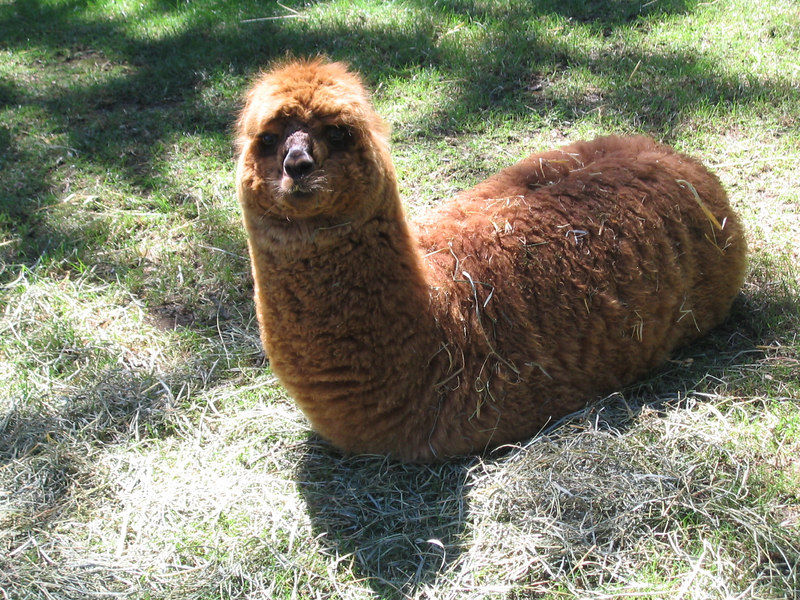
\includegraphics[width=0.75\textwidth]{vip1066720.jpg}
	\end{center}
	\caption{{\em !`Cuidado! !`Las llamas son muy peligrosas!}\cite{de0u}}
\end{figure*}

\section{Ad-hoc Thread Communication}

Inter-thread communication can be much more ad-hoc in kernel-space than in user-space\hspace{0in}\cite{datacollider}, and a systematic testing framework needs to be aware of all the kernel's synchronisation idioms.

\begin{itemize}
	\item {\bf Avoiding reliance on message-passing.} Some systems for user-space systematic testing require that threads communicate only by message-passing, to better track the concurrency relationships between thread transitions\cite{dbug-ssv}. With few exceptions\cite{barrelfish}, kernels do not rely on message-passing as a primary communication mechanism, and to be compatible with the kernels of today, a testing framework must allow for less idealised state-sharing (Section~\ref{sec:components-memory}).
	\item {\bf Recognising blocked threads.} It is difficult to detect when threads are ready to do useful work. Even if notionally runnable, they may be waiting in a yield loop (Sections~\ref{sec:using-annotations} and \ref{sec:future-linux}). A tool that did not recognise this might decide to attempt to run that thread over and over, and get stuck because the other threads would never be allowed to make progress.
	\item {\bf Thread lifecycle tracking.} It is also difficult to demarcate threads' lifecycles: when a new thread gets created, when is it available to run? and when a thread is exiting, at what point does it stop running code (Section~\ref{sec:using-annotations})? In user-space, these boundaries are defined by the system call instructions, but in kernel-space, the boundary is fuzzier.
	\item {\bf Use of virtual memory.} The kernel's complete control over the machine's virtual memory system means a system for tracking memory accesses must be aware of changing virtual memory mappings (Section~\ref{sec:using-requirements}).
\end{itemize}

\section{Kernel Design}
\label{sec:challenges-design}

One challenge particular to the context of 15-410 is that the kernels Landslide must be able to test may all use slightly different implementations to achieve the same goals. For Landslide to be generally applicable to (almost) any kernel that students may submit, it must make some abstract assumptions about the kernel design which are compatible with many different implementations.

In certain avenues of future work (Section~\ref{sec:future-linux}), remaining agnostic of most implementation details becomes less of an issue. For example, if we target Landslide to Linux, it is unlikely that core scheduler or interrupt-handling behaviour will change for as long as Landslide remains useful for finding bugs. In 15-410, however, repeated re-targetting is a necessity.

We built Landslide to be compatible with multiple designs for the following major scheduling behaviours:

\begin{itemize}
	\item {\bf Runqueues}: Does the kernel store the currently-running thread on the runqueue, or is it removed and stored separately?
	\item {\bf Mutexes}: When a thread blocks on a mutex, is it left on the runqueue in a yield-loop, or is it explicitly descheduled? In yield-looping mutexes, when do blocked threads become ``unblocked'', notionally? (This might happen before the blocked thread runs next.)
	\item {\bf Idling}: Does the kernel have an explicit idle thread, or is there an idle loop that runs on the stack of whatever thread was last running? Do explicit idle threads run their idle loop in userspace or in kernelspace?
	\item {\bf Thread Creation}: When a thread is newly forked, is it placed onto the runqueue for later, or is it context-switched to immediately? Do just-forked threads begin life through the usual context-switch-return path, or is there a special path for that?
	\item {\bf Test Lifecycle}: Even apart from running on a particular input that the user wishes to test, the kernel may need to perform extra work irrelevant to the test, such as initialisation (e.g. the bootup process) and housekeeping (e.g. cleaning up dead processes). Which parts of this work should be included or excluded in the test?
\end{itemize}

Conversely, Landslide needs to make some assumptions about scheduling behaviour, in order for its control over scheduling to work:

\begin{itemize}
	\item {\bf Timer ticks control ``runnable'' threads.} With the exception of a non-preemptible ``scheduler lock'', and yield-looping mutexes (both of which must be instrumented by the user), a thread's presence on the runqueue indicates that a finite number of timer interrupts in succession will eventually cause it to run.
	\item {\bf No idling when progress can be made.} The kernel must not enter its idle loop (whether in an explicit idle thread or no) when the kernel is not truly idle. Landslide uses the idle loop to detect when a test begins/ends and to detect when all threads in a test are wedged.
\end{itemize}

%%%%%%%%%%%%%%%%%%%%%%%%%%%%%%%%%%%%%%%%%%%%%%%%%%%%%%%%%%%%%%%%%%%%%%%%%%%%%%%%
\chapter{Design and Implementation}
%%%%%%%%%%%%%%%%%%%%%%%%%%%%%%%%%%%%%%%%%%%%%%%%%%%%%%%%%%%%%%%%%%%%%%%%%%%%%%%%
\label{sec:design}

In this chapter we describe Landslide's implementation in detail. Section~\ref{sec:model} outlines the testing model on top of which Landslide's exploration mechanisms are built. Section~\ref{sec:components} describes the individual components within Landslide. Section~\ref{sec:techniques-bugs} describes Landslide's metrics for identifying bugs. Section~\ref{sec:techniques-por} describes how Landslide achieves effective state space reduction. Section~\ref{sec:techniques-feedback} describes the debugging feedback Landslide provides to the user when bugs are encountered.

\revision{
\section{Landslide's View of the World}
\label{sec:model}

Landslide's model for applying systematic exploration in kernel-space is comprised of four key points, which we overview here.

\subsection{Simulated Execution}
\label{sec:model-simics}

Landslide is implemented as a module for Simics\cite{simics}, a full-system x86 emulator. When running the kernel, Simics calls into Landslide once every time the kernel executes an instruction or performs a memory read or write. Landslide uses this information, in conjunction with the user-provided instrumentation, to maintain its internal representations of the state of the guest kernel.

Landslide makes use of Simics ``bookmarks'', a feature which enables checkpointing and restoring the execution state of the guest kernel, to implement backtracking when the end of each branch in the decision tree is reached.

\subsection{Timer-Driven Scheduling}
\label{sec:model-timer}

In this work, we focus specifically on nondeterministic scheduling driven by timer interrupts. Landslide assumes that timer interrupts are the only source of nondeterminism for the guest kernel, so controlling when they occur theoretically allows for complete control over the concurrent behaviour of the test case. In future work (Section~\ref{sec:future-drivers}), we may also address causes of non-determinism more complex than timer-driven thread scheduling, such as interrupts and data I/O from peripheral devices.

Landslide needs to impose some requirements on the guest kernel's scheduling behaviour, in order for its control over scheduling to work:

\begin{itemize}
	\item {\bf Timer ticks control ``runnable'' threads.} With the exception of a non-preemptible ``scheduler lock'', and yield-looping mutexes (both of which must be instrumented by the user), a thread's presence on the runqueue indicates that a finite number of timer interrupts in succession will eventually cause it to run.

	Landslide treats the sleep queue no differently from the runqueue when deciding which threads are runnable. The guest kernel will treat it differently, but since sleeping for a predetermined amount of time is never an appropriate way to solve race conditions, Landslide treats sleeping threads as notionally runnable. This fits directly into its model that runnable threads are ones that can be caused to run with a finite number of timer ticks in succession.
	\item {\bf No idling when progress can be made.} The kernel must not enter its idle loop (whether in an explicit idle thread or no) when the kernel is not truly idle. Landslide uses the idle loop to detect when a test begins/ends (test lifecycle tracking) and to detect when all threads in a test are wedged (bug detection).
\end{itemize}

Section~\ref{sec:components-inflight} gives more detail about how Landslide abstracts raw timer interrupts into the ability to cause arbitrary threads to run.

\subsection{False-Negative-Oriented Bug Detection}
\label{sec:model-bugs}

% A healthy dose of snark.
Without a formal specification of the internals of the guest kernel's implementation\cite{sel4}, it is impossible to identify both soundly and completely when a behaviour that constitutes a ``bug'' arises during a test case's execution.
Landslide's bug reporting is false-negative oriented, meaning that it does not check for suspicious behaviours that might indicate underlying bugs, so it may report that it found no bugs even if some existed. If Landslide does report a bug, though, it is almost certainly correct. Section~\ref{sec:techniques-bugs} details the conditions Landslide uses to identify when something has gone wrong.

\subsection{User-Assisted State Space Reduction}
\label{sec:model-user}

In addition to Dynamic Partial Order Reduction (DPOR) for automated state space reduction, Landslide relies on the user's guidance to help mitigate the possible combinatorial explosion of thread interleaving possibilities. This manifests in two ways:

\begin{itemize}
	\item {\bf Decision point selection.} Landslide provides an interface for the user to manually limit identification of decision points to only ``relevant'' modules of the kernel, thereby only generating thread interleavings around points within those modules.
	\item {\bf Memory conflict selection.} Landslide also provides a mechanism for ignoring shared memory conflicts on certain common data structures (especially those accessed in every thread transition, such as the scheduler queues), to enable DPOR to achieve greater reduction. Intuitively, this represents sacrificing the ability to find races around those data structures to make searching other components more feasible.
\end{itemize}

We advocate relying on the user for such information because the user need only understand the basics of their kernel design (which is difficult for Landslide to guess) while not knowing in advance what bugs are being looked for (which Landslide is able to provide). We claim that this combination of the user's knowledge and Landslide's testing mechanisms leads to an effective usage dynamic, in which the user ``steers'' Landslide towards focused search spaces that are more likely to find bugs.

The interfaces by which the user provides this information are documented in Section~\ref{sec:using-customise}.
}

\section{Components of Landslide}
\label{sec:components}

In this section we briefly describe each major component of Landslide.

\begin{figure}[h]
	\centering
	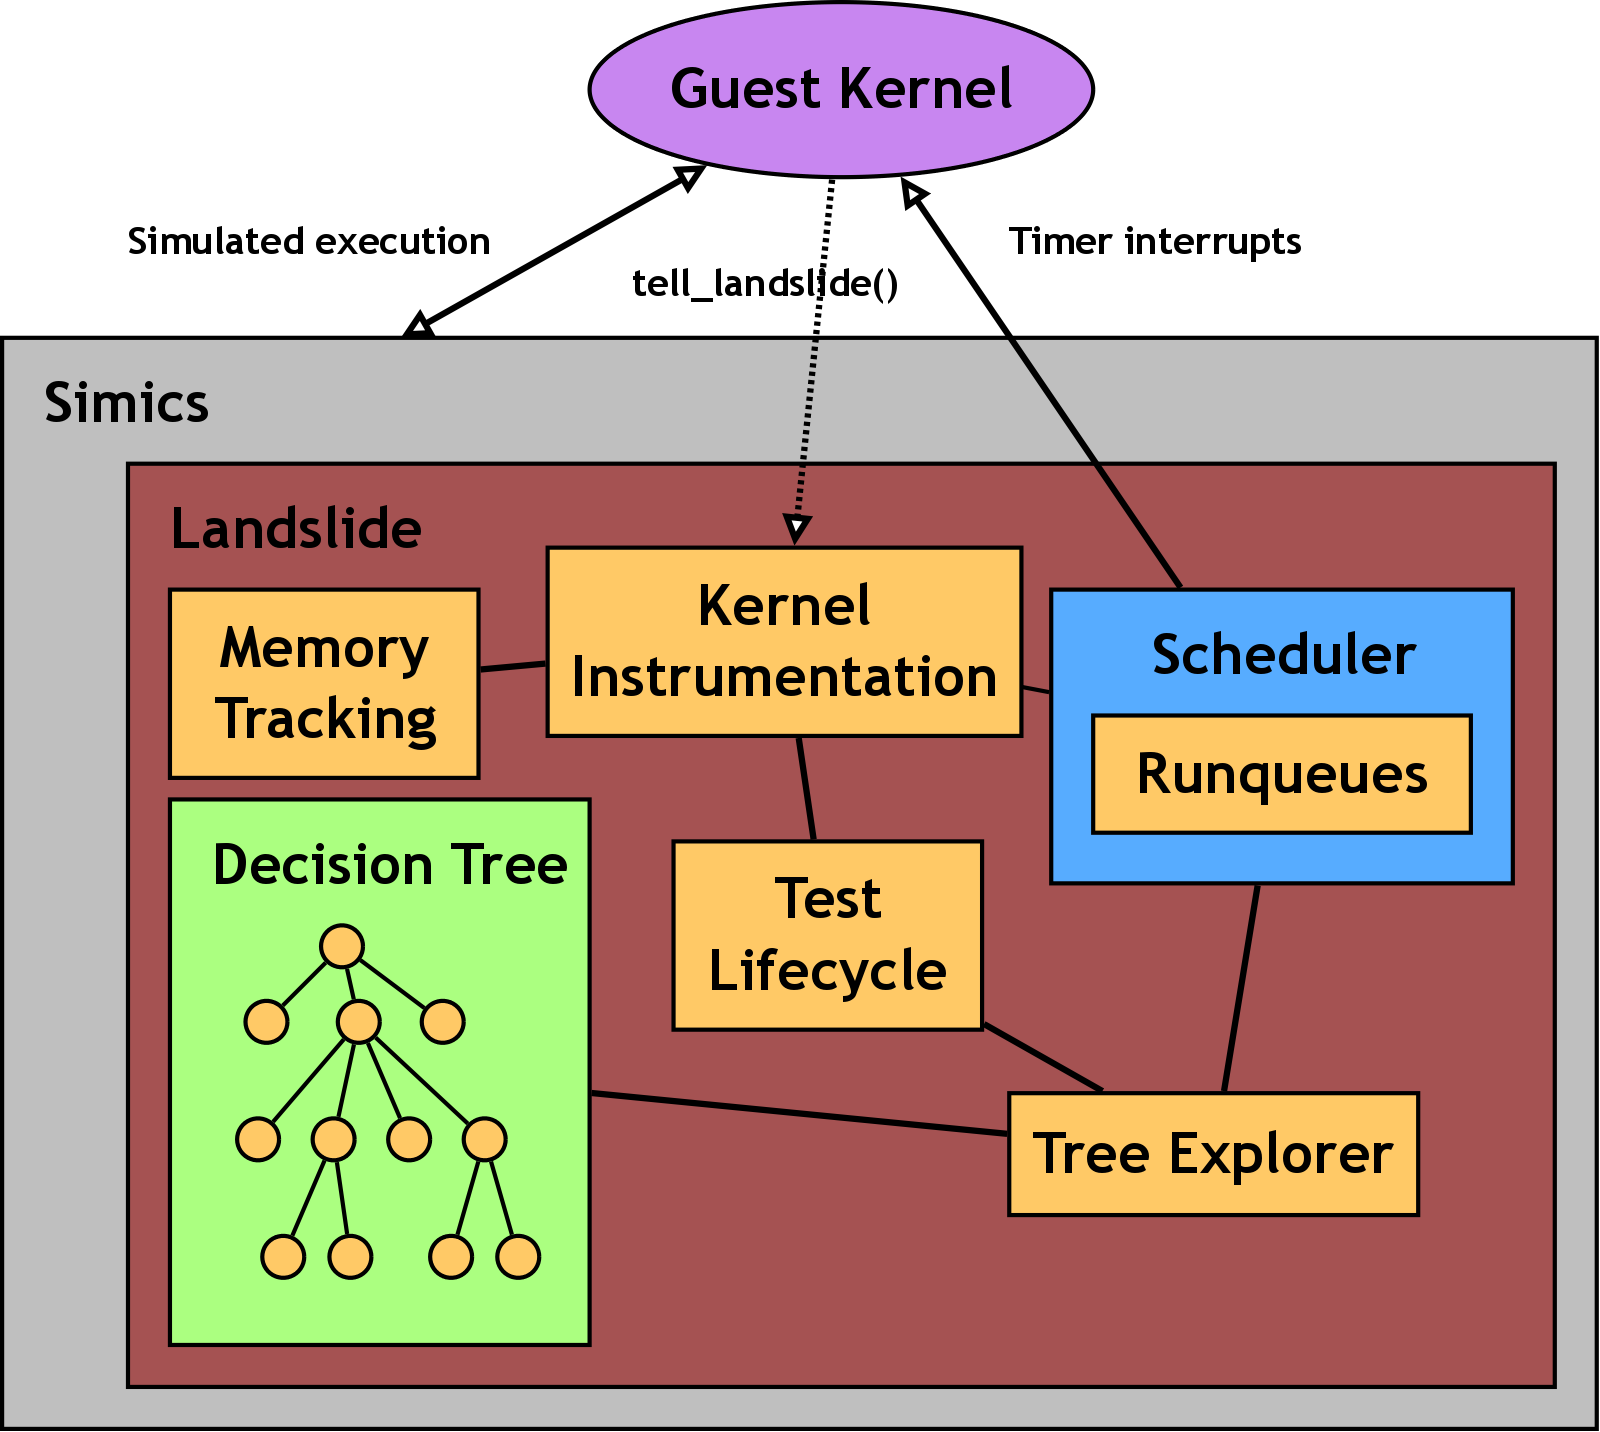
\includegraphics[width=0.75\textwidth]{landslide.png}
	\caption{A simple visualisation of Landslide and its components, and how they interact with the guest kernel.}
	\label{fig:landslide}
\end{figure}

\subsection{Kernel Instrumentation}
\label{sec:components-kern}

The kernel instrumentation serves as the glue between what the guest kernel is doing and Landslide's understanding of the guest kernel's state.

\begin{itemize}
	\item {\bf User-provided instrumentation.} Some parts of the kernel may be written in any number of ways, and hence require the user's assistance for Landslide to understand. The user-provided instrumentation, described in detail in Section~\ref{sec:using-instrumenting}, informs Landslide about thread-related lifecycle and scheduling events and the anatomy of the kernel's scheduler.
	\item {\bf Automatic instrumentation.} All Pebbles kernels have some things in common (largely due to the common starter code provided for the class project), and Landslide's build system is able to automatically instrument certain parts of the kernel. This instrumentation informs Landslide about the dynamic memory allocator, common library functions such as \texttt{panic}, and certain aspects of the kernel's executable format.
\end{itemize}

\subsection{Scheduling}
\label{sec:components-sched}

The Landslide scheduler is responsible for keeping track of which threads exist in the guest kernel: which are runnable at any given time, and when they are created and destroyed.

It maintains a ``mirror image'' of the guest kernel's scheduler state in the form of three queues, a pointer to the currently-running thread, and a pointer to the previously-running thread. The queues are the {\em runqueue}, containing the runnable threads, the {\em sleep queue}, containing threads which become runnable after a certain number of timer ticks, and the {\em deschedule queue}, which might not correspond to a data structure in the guest kernel, but contains all other threads that exist on the system, which are not runnable for whatever reason.

The Landslide scheduler also tracks which important actions each thread is performing. These actions are {\em forking}, {\em vanishing}, and {\em sleeping}, which are described in the next section, and also {\em in\_timer\_handler} and {\em in\_context\_switch}, which express what type of context switch a given thread may be performing, and are useful for both thread scheduling (Section~\ref{sec:components-inflight}) and detecting voluntary reschedules (Section~\ref{sec:components-arbiter}).\footnote{
There are also other minor actions: {\em readlining}, used to track test lifecycle (Section~\ref{sec:components-test}), {\em just\_forked}, used for special-case context switch behaviour (Section~\ref{sec:components-arbiter}), and also several flags for tracking mutex lock/unlock events.}

\subsubsection{Thread Lifecycle Tracking}

\begin{algorithm}[t]
	\footnotesize
	\begin{algorithmic}
		\State {\em Per-thread state.}
		\State bool forking, sleeping, vanishing, in\_timer\_handler;
		\State int current\_tid;
		\\
		\Function{handle\_tell\_landslide\_forking}{}
			\State forking $\gets$ true;
		\EndFunction
		\\
		\Function{handle\_tell\_landslide\_sleeping}{}
			\State sleeping $\gets$ true;
		\EndFunction
		\\
		\Function{handle\_tell\_landslide\_vanishing}{}
			\State vanishing $\gets$ true;
		\EndFunction
		\\
		\Function{handle\_tell\_landslide\_thread\_switch}{int new\_tid}
			\If {!in\_timer\_handler}
				\If{sleeping}
					\State {\sc add\_to\_sleep\_queue}(current\_thread);
					\State sleeping $\gets$ false;
				\ElsIf{vanishing}
					\State {\sc destroy\_thread}(current\_tid);
					\State vanishing $\gets$ false;
				\ElsIf{forking}
					\State {\sc create\_thread}(new\_tid);
					\State forking $\gets$ false;
				\EndIf
			\EndIf
			\State {\sc update\_current\_thread}(new\_tid);
		\EndFunction
	\end{algorithmic}
	\caption{Landslide's scheduler's routines for tracking thread lifecycles. These routines are invoked each time the guest kernel calls one of the \texttt{tell\_landslide} annotations.}
	\label{alg:tell-landslide}
\end{algorithm}

The Landslide scheduler relies on the guest kernel informing it about certain important events in the thread lifecycle. The guest kernel does this by means of annotations (which are described in Section~\ref{sec:using-annotations}). Algorithm~\ref{alg:tell-landslide} shows how Landslide handles these annotations internally.\footnote{
There are also cases for the runqueue annotations, \texttt{tell\_landslide\_on\_rq} and \texttt{tell\_landslide\_off\_rq}, which we omit for brevity. One important note is that the routine for \texttt{tell\_landslide\_on\_rq} must also check the ``forking'' flag, in case the kernel's \texttt{fork} implementation does not immediately switch to the new thread but instead adds it to the runqueue for later.}

\subsubsection{Thread Scheduling}
\label{sec:components-inflight}

Finally, the Landslide scheduler is responsible for managing involuntary preemptions, causing arbitrary threads to begin running in place of the current one (as chosen at decision points and the ends of branches by the explorer, Section~\ref{sec:components-explore}).

\begin{algorithm}[t]
	\footnotesize
	\begin{algorithmic}
		\State {\em Global scheduler state.}
		\State bool schedule\_in\_flight;
		\State int target\_tid;
		\\
		\State {\em Per-thread state. (Updated elsewhere.)}
		\State bool in\_timer\_handler, in\_context\_switch;
		\State int current\_tid;
		\\
		\Function{scheduler\_update}{int pc}
			\If{schedule\_in\_flight}
				\State {\sc assert}(in\_timer\_handler || in\_context\_switch);
				\If { {\sc kernel\_exiting\_timer}(pc) || (!handling\_timer \&\& {\sc kernel\_exiting\_context\_switch}(pc))}
					\State {\em The kernel has just finished rescheduling and is about to resume normal thread execution.}
					\If {current\_tid != target\_tid}
						\State {\em The kernel switched to an undesirable thread. Keep the schedule operation ``in-flight''.}
						\State {\sc cause\_timer\_interrupt}();
					\Else
						\State {\em The in-flight schedule is ``landing''.}
						\State schedule\_in\_flight $\gets$ false;
					\EndIf
				\EndIf
			\ElsIf{{\sc need\_to\_preempt}()}
				\State target\_tid $\gets$ {\sc choose\_new\_thread}();
				\State schedule\_in\_flight $\gets$ true;
				\State {\sc cause\_timer\_interrupt}();
			\EndIf
		\EndFunction
	\end{algorithmic}
	\caption{Landslide's scheduling algorithm. This procedure for updating Landslide's state is executed once per instruction, with a corresponding value for \texttt{pc} (the program counter) each time. The predicates on \texttt{pc} are part of the kernel instrumentation (Section~\ref{sec:components-kern}).}
	\label{alg:inflight}
\end{algorithm}

Though we define timer interrupts as the only source of non-determinism in our environment, it is more useful to view the concurrent behaviour with a higher-level abstraction, in terms of the set of runnable threads and the ability to preempt the currently-running thread with any different runnable one.

Landslide's scheduling technique, called the {\em schedule in-flight}, involves successive triggering of timer interrupts to trigger context switches until the desired thread begins to run. Algorithm~\ref{alg:inflight} shows how Landslide makes this happen.

One alternative simpler method would be, when triggering a timer interrupt, to tell the guest kernel explicitly which thread should be run next. This would require the kernel programmer to write extra code in their timer handler and/or context switcher. We chose the ``in-flight'' approach instead, because it does not require additional kernel modifications.

\subsection{Memory Tracking}
\label{sec:components-memory}

Landslide maintains a mirror image of the guest kernel's dynamic allocation heap, so it can know at any point which memory ranges are allocated and which ranges used to be allocated but now are freed. This set is updated each time the guest kernel calls \texttt{malloc} or \texttt{free}.

Landslide also maintains a set of shared memory accesses made since the last decision point, for use with Partial Order Reduction (Section~\ref{sec:por-independence}). Whenever the guest kernel accesses memory in its heap or in its global data regions, Landslide adds the address of the access to the set, with a flag indicating whether it was a read or a write. (If the address was already present, and the recorded access was a read and the current access is a write, we upgrade the recorded access to a write. Otherwise if the address was already present, we do nothing.)

Landslide ignores shared memory accesses from the kernel's dynamic allocator itself, and it also ignores shared memory accesses from the components of the kernel's scheduler which run every transition (Section~\ref{sec:por-independence}).

When Landslide reaches a decision point, this accumulated set is copied in the decision tree (Section~\ref{sec:components-explore}), and reset to empty before continuing execution.

\subsection{The Arbiter}
\label{sec:components-arbiter}

The arbiter identifies points during execution that should count as decision points. The selection is mainly controlled by the user, during the annotation and configuration process. In addition, the arbiter also automatically identifies {\em voluntary reschedules}, which comprise the ``minimal necessary set'' of decision points.

A voluntary reschedule is identified when:
\begin{itemize}
	\item The previously-running thread entered the context switcher without first entering the timer interrupt handler,
\end{itemize}

and {\em any one} of the following:
\begin{itemize}
	\item The currently-running thread was handling a timer interrupt, and exits the {\em timer interrupt handler}.
	\item The currently-running thread was not handling a timer interrupt, and exits the {\em context switcher}.
	\item The currently-running thread was {\em just forked} (i.e, it has never run before), and hence may never exit either the timer handler or context switcher.
\end{itemize}

It is always necessary to identify a decision point during a voluntary reschedule, to maintain the invariant that each transition between decision points is comprised of the execution of only one thread.

In future work (Section~\ref{sec:future-new}), the arbiter may also automatically identify extra decision points, such as conflicting shared memory accesses.

\subsection{The Explorer}
\label{sec:components-explore}

The explorer maintains a representation of the current branch of the decision tree. It is responsible for checkpointing the state of both Landslide and the guest kernel at each decision point, deciding at the end of the test which branch of the tree to execute next (i.e., selecting which decision point should have been decided differently), and backtracking to appropriate points in the test's execution.

At each decision point, Landslide creates a new node in the decision tree. It stores the TID of the thread that was chosen, the state of the scheduler (which threads are on the runqueue), the state of the heap and the accumulated set of shared memory accesses, and a stack trace of the thread that was running.

\subsection{Test Lifecycle}
\label{sec:components-test}

\begin{figure}[h]
	\begin{center}
		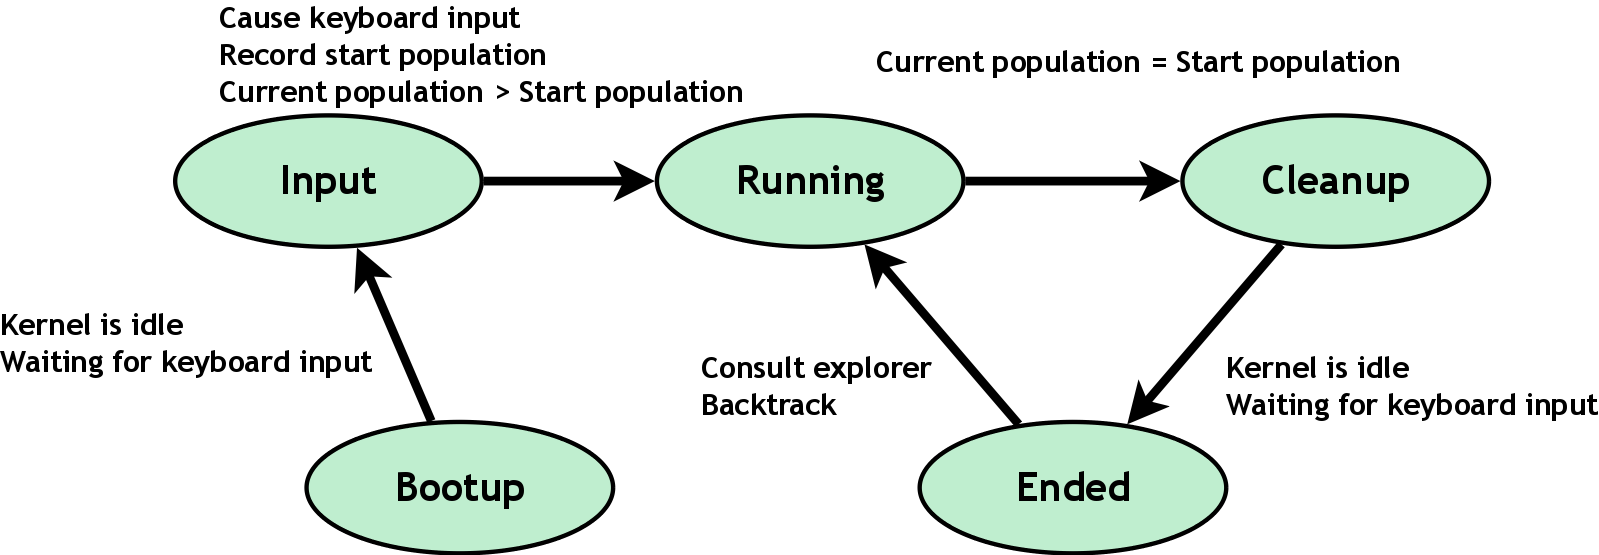
\includegraphics[width=0.8\textwidth]{teststate.png}
	\end{center}
	\caption{The test lifecycle state machine.}
	\label{fig:teststate}
\end{figure}
Landslide knows the state of the test case through a simple state machine, which is updated with information about the number of threads currently on the system, the number of threads on the runqueue, the state of the idle thread (if it exists), and whether or not the shell is waiting for keyboard input.

The state machine relies on certain information provided by the scheduler (Section~\ref{sec:components-sched}).

\begin{itemize}
	\item {\bf Is the shell waiting for keyboard input?} In general, the shell only waits for keyboard input when the kernel is ready for the user (or Landslide) to cause a test to run, or after the test has finished and a new one could be run.
		However, the shell may sometimes be waiting for keyboard input while other threads have some work to do (for example, the init process might not yet have reaped a reparented child process), and this work may be affected by race conditions during the test, so we need to include it in the test as well. For these cases an additional check is needed.
	\item {\bf Is the kernel idling?} This indicates whether any work is left to be done during bootup or during teardown.
	\item {\bf How many threads currently exist on the system?} This indicates whether the test has begun running.
\end{itemize}

The states in the test lifecycle, and the rules for transitioning between them, are as follows.

\begin{enumerate}
	\item {\bf Bootup.} Initial state. When the kernel is idling and the shell is waiting for keyboard input, advance state.
	\item {\bf Keyboard input.} Record the current thread count (the ``start population''). Generate keystrokes to cause the desired test case to run.
		When the current thread count is greater than the start population, advance state.
	\item {\bf Test running.} Begin constructing the decision tree here (since it is pointless to backtrack to before the test begins). When the current thread count equals the start population, advance state.
	\item {\bf Test cleanup.} The test processes have exited, but some housekeeping may yet remain. When the the kernel is idling and the shell is waiting for keyboard input, advance state.
	\item {\bf Test ended.} Invoke the explorer (Section~\ref{sec:components-explore}) to decide whom to rewind, and backtrack (to step 3).
\end{enumerate}

Figure~\ref{fig:teststate} depicts the states and transitions visually.

%\subsection{Stack Tracing}
% FIXME

\section{Identifying Bugs}
\label{sec:techniques-bugs}

In order to identify when the guest kernel has done something incorrect, Landslide performs several different types of checks, some accurate but noncomprehensive, and some heuristic-based.

\subsection{Definite Bug-Detection Conditions}

\begin{enumerate}
	\item {\bf Kernel panic bugs.} If the kernel invoked \texttt{panic}, it detected its own bug, and Landslide need do nothing but report it.
	\item {\bf Use-after-free bugs.} Whenever the kernel accesses memory in the heap (when not in the dynamic allocator itself), Landslide verifies that the address is within an allocated range. If not, Landslide proclaims the access to be illegal.\footnote{In the same way, Landslide also detects calls to \texttt{free} on blocks that were already freed or never allocated at all.}
	\item {\bf Deadlock bugs.} If Landslide finds no runnable threads on the runqueue,\footnote{Except for idle, if it exists.} or if it detects a cycle of threads blocked on each other, it declares that the kernel has deadlocked.
\suspend{enumerate}

\subsection{Probable Bug-Detection Conditions}

\resume{enumerate}
	\item {\bf Memory leak bugs.} Landslide records the state of the heap before the test case begins, and compares it to the state of the heap after the test case ends. If memory allocated during the test was not freed, Landslide assumes that it was leaked.
		(Some kernel designs may legitimately behave this way, so this bug-check may be disabled when testing such kernels.)\footnote{There is, of course, much room for improvement in this metric, but it is not part of the research contribution.}
	\item {\bf Infinite loop bugs.} Landslide judges whether the kernel has entered an infinite loop by comparing the current state of the decision tree to past executions of the same test case.
	\begin{itemize}
		\item While exploring the decision tree, Landslide computes the average number of instructions executed between two consecutive decision points. If at any point the current number of instructions executed since the most recent decision point exceeds this average times a constant factor (arbitrarily chosen to be 2000), Landslide assumes the kernel must have gotten stuck in an infinite loop.
		\item Landslide also computes the average number of decision points in each branch of the decision tree (the average ``branch depth''). If the depth of the current branch ever exceeds this average times a constant factor (arbitrarily chosen to be 20), Landslide assumes the kernel must have gotten stuck in an infinite loop.
	\end{itemize}
\end{enumerate}

\section{Partial-Order Reduction}
\label{sec:techniques-por}

We make use of Dynamic Partial-Order Reduction (DPOR), the state-space pruning algorithm presented in \cite{dpor}. DPOR requires two sets to be computed that describe the concurrency relationship between transitions: the happens-before relation, and the memory independence relation. Here we discuss the specifics of implementing these in our environment.

\subsection{Happens-Before Relation}

\revision{The happens-before relation expresses for each pair of transitions whether executing the first one is required to ``enable'' the second one. In order to establish the relation,} Landslide uses the state of the scheduler runqueues (Section~\ref{sec:components-sched}), which are snapshotted at every decision point (Section~\ref{sec:components-explore}).

Unfortunately, a thread's presence or absence on the scheduler runqueue does not necessarily correspond to whether it is {\em runnable} at any point. We identify three exceptions, as foreshadowed in Section~\ref{sec:challenges-design}:

\begin{itemize}
	\item {\bf Current thread not on runqueue.} If the currently-running thread is not stored on the runqueue, we identify it as runnable anyway (except in the special case of idle, as described below).
	\item {\bf Idle thread.} Some kernels may have an explicit idle thread and store it on the runqueue, with explicit code to skip over it if other threads are runnable. Hence, if the idle thread is on the runqueue (and/or the current thread), it is only runnable if no other threads are runnable.
	\item {\bf Yielding mutexes.} In kernels whose mutexes (or other synchronisation idioms) leave threads on the runqueue when they are notionally blocked, Landslide classifies such threads as not runnable.
\end{itemize}

Using this notion of runnability, the happens-before relation is established as follows. Let $X$ be a transition and $Y$ be a subsequent transition in a branch that was just explored, and $T_Y$ be the thread associated with $Y$. We say that $X$ {\em enables} $Y$ if $T_Y$ was not runnable immediately before $X$, but was runnable immediately after. Then, a transition $A$ happens-before a transition $B$ if $T_A$ is the same thread as $T_B$, if $A$ enables $B$, or if $A$ happens-before some transition $C$ that enables $B$.

\subsection{Memory Independence Relation}
\label{sec:por-independence}
The independence relation expresses which transitions do not read-and-write or write-and-write to the same shared memory addresses. Landslide computes this relation using the set of shared memory accesses described in Section~\ref{sec:components-memory}. We encountered two challenges pertaining to memory independence:

\begin{itemize}
	\item {\bf Always-accessed memory locations.}
		In kernel-space, every thread switch goes through common scheduler and context-switcher routines. These routines inevitably access scheduler data structures, such as the runqueue.\footnote{
		Another example is the timer tick counter: this global variable is not necessarily accessed every transition, because voluntary reschedules do not involve timer interrupts, but every involuntary preemption will cause a write to this counter.}
		If we include such memory accesses in the independence relation, it will result that all transitions conflict, and DPOR won't be able to achieve any reduction. To allow for state space reduction, we sacrifice our ability to find races involving these particular accesses by ignoring them. Currently we require the user to identify these locations as part of the instrumentation process, as described in Section~\ref{sec:using-config-landslide}.
	\item {\bf Freed memory poisoning.}
		A use-after-free bug happens whenever one thread accesses an address within an allocated block that another thread previously freed. Even if no other code makes a conflicting access to the same address after the \texttt{free}, the C idiom says that accessing dynamically-allocated memory after it has been freed is illegal no matter what.

		Hence, even if the second thread that freed the block never accesses the particular address that the first thread used, the second thread's \texttt{free} still logically conflicts with the first thread's access. Landslide addresses this by treating every call to \texttt{free} as a {\em write} access to every address within the freed block when computing shared memory conflicts.
\end{itemize}

\subsection{Soundness}

\revision{
Because we recommend using Landslide with coarse-grained decision sets, as opposed to mandating a decision point between every pair of shared memory accesses, it is possible for Landslide to overlook race conditions that require finer-grained interleavings to expose. In this way, Landslide's search is not ``sound'', but instead false-negative-oriented.

We do, however, claim that Landslide's search is sound in a different way: if the provided decision points are sufficient to express an interleaving that would expose a race, then Landslide will find it. That is, if Landslide is exploring an execution tree with bugs in some branches, it will eventually find a bug.

Dynamic Partial Order Reduction works by identifying ``evil ancestors'' for each transition in a branch after executing that branch. Intuitively, a transition's evil ancestor is another transition such that executing the test with the order of those two transitions reversed could cause different concurrent behaviour to arise.}
\cite{dpor} and \cite{dbug-retreat} present a partial order reduction algorithm in which only the first evil ancestor of each transition need be considered when identifying which alternate interleavings need to be explored.

\begin{figure}[h]
	\centering
	\begin{tabular}{cc}
	\subfloat[Race-free interleaving.]{
		\footnotesize
		\begin{tabular}{l|c|c|c|}
			\cline{2-4}
			& {\bf Thread 1} & {\bf Thread 2} & {\bf Thread 3} \\
			\cline{2-4}
			$A$ & \texttt{x=42;} & & \\
			$B$ & & \texttt{y=31337;} & \\
			\multirow{2}{*}{$C_1$} & & & \texttt{if (y==31337)} \\
			& & & \texttt{assert(x==42);} \\
			\cline{2-4}
		\end{tabular}
	} &
	\subfloat[Alternate interleaving explored with DPOR.]{
		\footnotesize
		\begin{tabular}{l|c|c|c|}
			\cline{2-4}
			& {\bf Thread 1} & {\bf Thread 2} & {\bf Thread 3} \\
			\cline{2-4}
			$A$ & \texttt{x=42;} & & \\
			$C_2$ & & & \texttt{if (y==31337)} \\
			$B$ & & \texttt{y=31337;} & \\
			\cline{2-4}
		\end{tabular}
	} \\
	\multicolumn{2}{c}{
	\subfloat[Buggy interleaving.]{
		\footnotesize
		\begin{tabular}{l|c|c|c|}
			\cline{2-4}
			& {\bf Thread 1} & {\bf Thread 2} & {\bf Thread 3} \\
			\cline{2-4}
			$B$ & & \texttt{y=31337;} & \\
			\multirow{2}{*}{$C_3$} & & & \texttt{if (y==31337)} \\
			& & & \texttt{assert(x==42);} \\
			$A$ & \texttt{x=42;} & & \\
			\cline{2-4}
		\end{tabular}
	}}
	\end{tabular}
	\caption{This sample code defeats a DPOR implementation that uses only the first evil ancestor if a decision point is not defined between the two lines of thread 3's code. The first interleaving is explored first; DPOR identifies transition $B$ as the first evil ancestor of $C_1$, and runs the second interleaving next, reordering them. In the second interleaving, $A$ is no longer a second evil ancestor of $C_2$, so the third interleaving is never explored, and the assertion failure is missed.}
	\label{fig:evil-ancestors}
\end{figure}

We found that implementing DPOR in this way violated our second notion of soundness, because it relies on the invariant that each transition contains only one inter-thread communication event (in kernel-space, this means a shared memory access).
\revision{However, a key point of Landslide's recommended usage pattern is to sacrifice maximally-fine-grained decision points for performance, and so multiple different shared memory conflicts may happen in each transition.} Figure~\ref{fig:evil-ancestors} demonstrates a counterexample to the soundness of identifying only one evil ancestor per transition given our usage pattern.

\revision{Instead, Landslide uses considers every evil ancestor of each transition when performing DPOR. This modification enables Landslide to avoid the problem presented in the figure, because it will identify both alternate interleavings after exploring the first one. We claim without certainty that this change restores the second notion of soundness to Landslide's search, and leave proving this property to future work.}

\section{Debugging Feedback}
\label{sec:techniques-feedback}

\begin{figure}[t]
	\begin{center}
		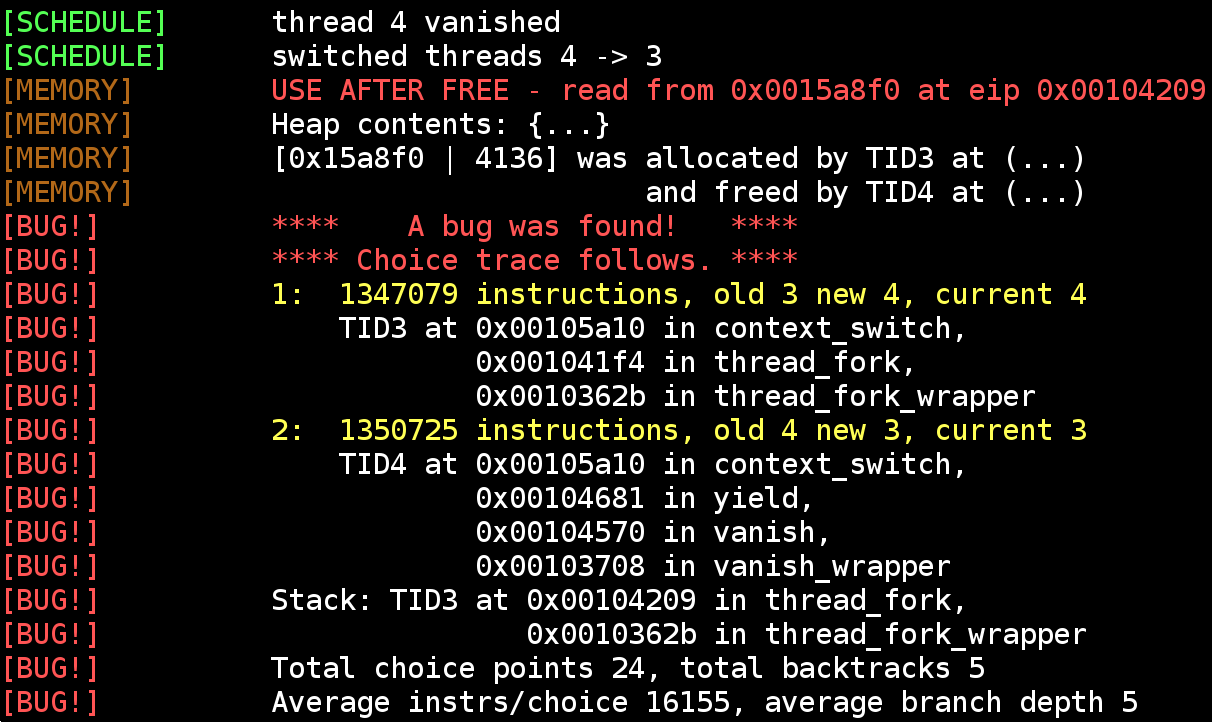
\includegraphics[width=0.95\textwidth]{found_a_bug.png}
	\end{center}
	\caption{A sample decision trace (with extraneous text trimmed) that Landslide generated using the \texttt{double\_thread\_fork} test case (Section~\ref{sec:using-tests}).}
	\label{fig:found_a_bug}
\end{figure}

In its unique position of control over when the kernel gets preempted and which thread gets scheduled at each context switch, Landslide has the capability to provide the user with detailed information about a test case's execution.
When Landslide determines that a bug was found, it immediately aborts exploration of the decision tree, and prints a {\em decision trace}: a comprehensive report of the particular interleaving of thread transitions that caused the bug to appear. Figure~\ref{fig:found_a_bug} depicts a simple decision trace for a use-after-free bug.

The decision trace explains each preemption or voluntary reschedule in the interleaving: which thread used to be running, which thread was chosen to run instead, and the stack trace of the former thread at the point from which it was switched away.

Landslide also prints the stack trace of the currently-running thread at the point where the bug was found, and (optionally) drops the user into the Simics debugging prompt. Depending on the nature of the bug found, Landslide also provides more detailed information:

\begin{enumerate}
	\item If the kernel has panicked, Landslide prints the message used in the panic/assertion.
	\item If a use-after-free bug is found, Landslide prints information about the most-recently-freed chunk containing the accessed address: the stack trace and TID both for when it was allocated and freed.
	\item If deadlock is detected, Landslide prints the cycle of TIDs that are blocked on each other.\footnote{This currently only works when using the annotations for yielding mutexes, though it is not difficult to implement more generally.}
	\item If a memory leak is suspected, Landslide prints how many bytes bigger the heap is after the test ended than when the test began.\footnote{Future feature: Printing when-allocated stack traces for each suspicious heap chunk.}
	\item If an infinite loop is suspected, depending on which heuristic was triggered, Landslide prints either the number of instructions since the last decision point (and the previous average) or the current branch depth (and the previous average).
\end{enumerate}

Landslide can also provide other useful information, even in cases where it did not find bugs, to help with the user's process of configuring decision points. Instead of exploring alternative interleavings, it can stop execution after the first interleaving and print out the set of decision points that were identified, along with the shared memory conflicts and happens-before relations for pairs of transitions between the decision points.

%%%%%%%%%%%%%%%%%%%%%%%%%%%%%%%%%%%%%%%%%%%%%%%%%%%%%%%%%%%%%%%%%%%%%%%%%%%%%%%%
\chapter{Using Landslide}
%%%%%%%%%%%%%%%%%%%%%%%%%%%%%%%%%%%%%%%%%%%%%%%%%%%%%%%%%%%%%%%%%%%%%%%%%%%%%%%%
\label{sec:using}
% TODO this whole section

\section{Kernel Requirements}
\label{sec:using-requirements}

\subsection{Scheduler Functionality}
\label{sec:using-requirements-sched}
% talk about different VM mappings when tracking shm conflicts

\section{Instrumenting Kernels with Landslide}

Here we describe the interface by which Landslide understands the execution of the guest kernel.

\subsection{In-Kernel Annotations}
\label{sec:using-annotations}

\subsection{Instrumenting Within Landslide}
\label{sec:using-student-c}


\section{Configuring Landslide's Behaviour}
\label{sec:using-customise}
\subsection{Decision Points}
\label{sec:using-decision}
\subsection{Search Parameters}
\label{sec:using-search}

\section{Test Cases}

We provide a set of test case programs for use with Landslide
% TODO: code listings in appendix

\subsection{Landslide-Friendly Test Characteristics}

\section{Interpreting Landslide's Results}
\label{sec:using-interpreting}


%%%%%%%%%%%%%%%%%%%%%%%%%%%%%%%%%%%%%%%%%%%%%%%%%%%%%%%%%%%%%%%%%%%%%%%%%%%%%%%%
\chapter{Evaluation}
%%%%%%%%%%%%%%%%%%%%%%%%%%%%%%%%%%%%%%%%%%%%%%%%%%%%%%%%%%%%%%%%%%%%%%%%%%%%%%%%
\label{sec:evaluation}

\revision{In evaluating Landslide, we sought to answer two overall questions.

\begin{itemize}
	\item Is Landslide an effective use of time by a developer seeking to find and understand race conditions in their code? How can Landslide be improved to improve the time tradeoff?
	\item When testing kernel code with a systematic testing framework, what overall use patterns are most effective for getting meaningful results? How can future work employ such patterns to build more sophisticated systematic testing tools for kernels?
\end{itemize}

To answer these questions, we evaluated Landslide in two ways.}
First, we conducted a user study with students of 15-410 during the spring 2012 semester, to understand the ease and difficulty of Landslide's user interface process, to understand how to polish it into a more useful debugging tool.
Second, we did a case study of six bugs in two kernels, investigating them in-depth to understand how systematic testing might best be harnessed to find bugs without in advance knowing the decision set necessary to expose them.

\section{User Experience}
\label{sec:eval-studence}

To evaluate the experience of non-expert users working with Landslide, we met with 5 groups of students in 15-410 (9 students in total) during the final week of the kernel project in spring 2012, and had them use Landslide with their own kernels. \revision{Additionally, one former 15-410 Teaching Assistant (TA) participated in the study.}

In order to garner student interest in Landslide, the author gave a lecture in 15-410 on systematic exploration in general and on Landslide specifically during the second-to-last week of the kernel project.\footnote{
The lecture slides are available at \url{http://www.cs.cmu.edu/~410-s12/lectures/L30_Landslide.pdf}, and at \url{http://bblum.net/landslide-lecture.pdf}, and at \url{http://www.contrib.andrew.cmu.edu/~bblum/landslide-lecture.pdf}.}

We wished to measure which phases of using Landslide are most time-consuming, so we asked students \revision{in intervals between 30 and 60 minutes} to record the amount of time they had spent doing each phase:

\begin{enumerate}
	\item Annotating their kernel (Section~\ref{sec:using-annotations}).
	\item Implementing instrumentation within Landslide (Section~\ref{sec:using-student-c}).
	\item Fixing problems encountered getting Landslide to run, such as editing their kernel to meet Landslide's requirements and debugging incorrect instrumentation.
	\item Customising Landslide's search parameters such as decision points (Section~\ref{sec:using-customise}).
	\item Analysing the output from bugs that Landslide found.
\end{enumerate}

We also wanted descriptive feedback, to evaluate which specific parts of the process of using Landslide need improved. We asked students to write brief remarks whenever they recorded amounts of time spent, and also after they were finished to answer the following questions.

\begin{itemize}
	\item Were you able to get Landslide to work with your kernel (i.e., run through a minimal exploration tree completely)? If so, how long did it take, from sitting down to getting it to work? If not, did your kernel do something that was incompatible with Landslide, or were you unable to get the instrumentation right for some other reason?
	\item Did you find bugs while using Landslide, that you imagine would have been very hard to find otherwise? Did Landslide's output help you understand what caused them?
	\item Were you able to get Landslide to say ``you survived!'' with custom decision points? Did you think the set of decision points you used for this provide a strong guarantee about the absence of races?
	\item Describe your experience configuring the set of decision points. What was intuitive, obvious to do? Did you feel stuck at any point, not knowing where to go next?
	\item Was there anything you wanted to make Landslide do that it didn't support?
\end{itemize}

Finally, we briefly studied each bug that the students found: whether they were deterministic or race conditions, whether they were deep unsolved concurrency problems or simple oversights, and the complexity of the necessary fixes.

\revision{Of five student groups that we worked with during the user study, four groups completed the instrumentation process and got Landslide to explore at least a minimal decision tree. (A minimal decision tree is one resulting from decision points only on voluntary reschedules, which Landslide automatically identifies.)}

\subsection{Time Breakdown}

\newcommand\asdf[1]{\hspace{-0.05in}\footnotesize\bf{#1}\hspace{-0.05in}}
\revision{
\begin{table}[t]
	\begin{center}
	\small
	\begin{tabular}{|l||c|c|c|c|c|c||c|c|}
		\hline
		\multirow{2}{*}{\bf Group} & \multicolumn{6}{|c||}{\bf Minutes spent doing\dots} & \multicolumn{2}{|c|}{\bf Total time spent} \\
		\cline{2-9}
		& \asdf{annotating} & \asdf{config} & \asdf{student.c} & \asdf{fixing} & \asdf{customising} & \asdf{found races} & \asdf{required} & \asdf{refinement} \\
		\hline \hline
		% ntaha/jmchow
		\multirow{2}{*}{Group 1} & 35 & {\footnotesize \em N/A} & {\footnotesize \em N/A} & 5 & {\footnotesize \em N/A} & {\footnotesize \em N/A} & {\footnotesize \em N/A} & {\footnotesize \em N/A} \\
		\cline{2-9}
		& 5 & 30 & 10 & 100 & {\footnotesize \em N/A} & {\footnotesize \em N/A} & 145 & {\footnotesize \em N/A} \\
		\hline
		% echo/margaret
		\multirow{2}{*}{Group 2} & 20 & 30 & 10 & 80 & {\footnotesize \em N/A} & 10 & 140 & 10 \\
		\cline{2-9}
		& 15 & 45 & 30 & 60 & {\footnotesize \em N/A} & 30 & 150 & 30 \\
		\hline
		% tpassaro
		\multirow{2}{*}{Group 3} & 15 & 10 & 5 & 60 & 30 & 30 & 90 & 60 \\
		\cline{2-9}
		& 15 & 10 & 5 & 60 & 30 & 30 & 90 & 60 \\
		\hline
		% pjumde
		\multirow{2}{*}{Group 4} & 10 & 42 & 3 & 5 & 30 & {\footnotesize \em N/A} & 60 & 30 \\
		\cline{2-9}
		& 15 & 35 & {\footnotesize \em N/A} & 5 & 35 & {\footnotesize \em N/A} & {\footnotesize \em N/A} & 35 \\
		\hline
		% apodolsk
		Group 5 & 50 & 15 & {\footnotesize \em N/A} & 15 & {\footnotesize \em N/A} & {\footnotesize \em N/A} & {\footnotesize \em N/A} & {\footnotesize \em N/A} \\
		\hline
		Former TA & 40 & 20 & 3 & 95 & {\footnotesize \em N/A} & 30 & 158 & 30 \\
		\hline
		\hline
		{\bf Average } & {\bf 22 } & {\bf 26.33 } & {\bf 9.43 } & {\bf 48.5 } & {\bf 31.25 } & {\bf 26 } & {\bf 119 } & {\bf 36.43} \\
		\hline
	\end{tabular}
	\end{center}
	\caption{Self-reported times spent by users on each phase while using Landslide. ``N/A'' indicates a student reported spending no time on a particular phase. ``Required'' indicates the sum of the times from the first four phases; ``refinement'' inducates the sum from the last two phases.
	``N/A'' indicates that a user did not report spending any time on a phase; the ``required'' field is ``N/A'' if any of its represented phases are, and ``N/A'' fields are not reflected in the averages.}
	\label{fig:student-times}
\end{table}
\begin{figure}[h]
	\center
	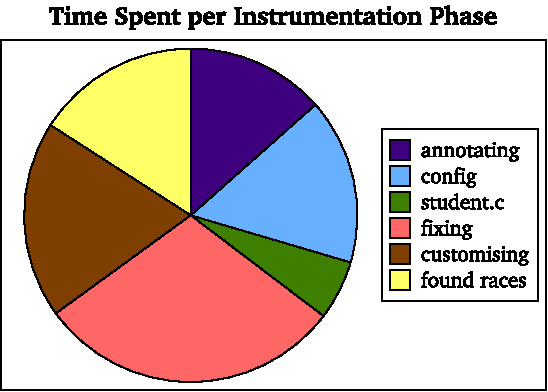
\includegraphics[width=0.5\textwidth]{graphs/studence-pie.pdf}
	\caption{Average time breakdown for each phase of instrumenting a kernel with Landslide, based on student self-reported times.}
	\label{fig:student-pie}
\end{figure}

While the students were using Landslide, we asked them at intervals from 30 to 60 minutes to record how much time they had spent on each phase of instrumenting and using Landslide.

\begin{itemize}
	\item {\bf Required instrumentation.} These phases represent work necessary to getting Landslide to work with a kernel at all.
	\begin{itemize}
		\item {\bf Annotating the kernel.} In this phase, the student modifies their kernel to use the provided annotations (Section~\ref{sec:using-annotations}).
		\item {\bf Writing the configuration file.} In this phase, the student fills out certain information about their kernel in \texttt{config.landslide} (Section~\ref{sec:using-config-landslide}).
		\item {\bf Instrumenting within Landslide.} In this phase, the student implements the two instrumentation functions in \texttt{student.c} (Section~\ref{sec:using-student-c}).
		\item {\bf Fixing instrumentation problems/crashing.} In this phase, the user repairs problems that arose due to incorrect instrumentation (or bugs in Landslide itself, in some cases).
	\end{itemize}
	\item {\bf Extra refinement.} These phases represent additional work to be done after successfully exploring a minimal decision tree. When such minimal exploration finds no bugs, such additional work is necessary to provide meaningful results.
	\begin{itemize}
		\item {\bf Customising decision points.} In this phase, the user configures Landslide to use decision sets more refined than the minimal one, in search of hard-to-find bugs (Section~\ref{sec:using-customise}).
		\item {\bf Investigating found race conditions.} In this phase, the user attempts to understand and fix bugs that Landslide found and reported.
	\end{itemize}
\end{itemize}

Table~\ref{fig:student-times} presents the time breakdown among phases that students experienced while using Landslide, visualised in Figure~\ref{fig:student-pie}. On average, students spent two hours getting Landslide to work with their kernels, and slightly more than half an hour customising the search and/or studying found bugs on top of that.

We consider the absolute values of these numbers largely artifacts of the user interface's quality (i.e., they could be improved with extra interface polishing, though they also currently present an upper bound). The relative values among phases, however, serve to give a notion of which phases were most difficult.

We do not think it useful to consider these times amortised over how many bugs were found for each group, because in general we do not know whether each group would have found more bugs with marginal extra effort, having already paid the initial cost of instrumenting. (The vanish/vanish bug we describe finding ourselves in Section~\ref{sec:eval-victory-races} serves as an example of this perennial possibility.)
Instead, we claim that the fact that Landslide found bugs for all groups who completed the required instrumentation proves its baseline effectivness as a debugging tool, and we note that the time tradeoff will become more worthwhile the more the user interface improves.
}

\subsection{Descriptive Feedback}
\label{sec:eval-feedback}

The students provided specific remarks which fell into two categories: issues with Landslide's user interface, and needing to change something in one's kernel to make it work with Landslide.

\subsubsection{User Interface Feedback}

For Landslide to be appealing as a debugging tool, we should improve the user interface (or the infrastructure, in some cases) to address the following issues.

\begin{itemize}
	\item {\bf Difficulty of debugging incorrect instrumentation.} When the user-provided annotations/instrumentation are incorrect, Landslide's error messages are difficult to understand, and often don't point to the real problem.
	\item {\bf Interpreting debugging output.} Some students reported the decision trace representation could be better. One student reported the output was easy to follow by ``tracing the life of the buggy thread'', which is an insight into the learning process we should capitalise on.
	\item {\bf Ease of configuring decision sets.} Most students seemed to find the process of adding more decision points intuitive. One reported, ``quick and effective at detecting basic bugs/races.'' \revision{While this interface could always be improved, of all the parts of the user experience, this process seems to need it least.}
	\item {\bf General feature wishlist.} The following features, of varying difficulty to implement, would have improved user experience overall.
		\begin{itemize}
			\item Being able to continue exploration after interrupting Simics to work with the debug prompt, instead of having to start over.
			\item Support for multiprocessor kernels.
			\item Cutting down overall simulation time.
		\end{itemize}
\end{itemize}

\subsubsection{Technical Feedback}

Students also described compatibility issues they faced between their kernels and Landslide, which required them to make certain changes to their kernels.
% FIXME: Say how we will address these issues?

\begin{itemize}
	\item {\bf Special-case context switch behaviour.} One kernel had a special context-switcher for the case when a thread was vanishing, which had to be special-cased in the instrumentation.
		Some kernels had different context switch designs for just-forked threads (as discussed in the ``Thread Creation'' bullet in Section~\ref{sec:challenges-design}), and Landslide's code had to be modified during the study to support different designs.
	\item {\bf Unexpected compiler optimisations.} Listing scheduler functions in \texttt{config.landslide} could be confusing if the compiler inlined them.
	\item {\bf Driver thread interfering with test lifecycle tracking.} One kernel (Pathos, the 15-410 reference kernel) had to be modified to ensure the keyboard thread ran once before the test started, which was not mandated by the kernel design. (If the thread didn't run, it would conflict with the population-tracking described in Section~\ref{sec:components-test}, and Landslide would not be able to detect when the test was over.)
	\item {\bf Kernel behaviour requirement violations.}
		The majority of groups needed to change their scheduling around the idle thread in order to meet the requirement that the kernel never run idle when progress could otherwise be made (Sections~\ref{sec:challenges-design} and \ref{sec:using-requirements-sched}).
		Also, one kernel had to have its custom memory allocator disabled, because Landslide only supports LMM, the allocator that 15-410 provides.

		\revision{The idle requirement is an inherent part of Landslide's model, whereas the dynamic allocator requirement could be replaced with a richer set of optional annotations.}
\end{itemize}

Additionally, two enterprising users found ways to avoid implementing the functions in \texttt{student.c} (Section~\ref{sec:using-student-c}). It is worth considering integrating these approaches into the recommended approach to eliminate the need for \texttt{student.c} entirely.
\begin{itemize}
	\item One student bypassed the \texttt{kern\_ready\_for\_timer\_interrupt} annotation by disabling their scheduler's preemption-disabling mechanism and replacing it with explicit disabling of interrupts. \revision{This caused the kernel to context switch every timer interrupt, so Landslide did not need to be aware of extra conditions that would cause the scheduler to ignore timer ticks.}
	\item The former TA was able to avoid the \texttt{kern\_current\_extra\_runnable} annotation by using the \texttt{on\_rq} and \texttt{off\_rq} annotations (Section~\ref{sec:using-annotations}) to express the ``abstract set of runnable threads'' (which included the currently-running thread, even though the runqueue didn't) instead of the literal runqueue itself. \revision{We did not advertise this method because we suspected students might make more mistakes instrumenting this way, but it might be worth advocating anyway for the sake of making the interface simpler.}
\end{itemize}

\subsection{Landslide Victories}
\label{sec:eval-victory}

Of the four groups that completed the required instrumentation, two found race conditions in their kernel. Additionally, Landslide helped all four groups find deterministic bugs: three groups had previously unknown problems with running the idle thread inappropriately, and the other group had a simple use-after-free.

We list how much progress each group made, and whether or not they found any bugs.

\begin{enumerate}
	\item % ntaha/jmchow
		Group 1 got Landslide to explore a minimal decision tree, and also explored \texttt{double\_wait} and \texttt{vanish\_vanish} with several combinations of different decision points around \texttt{mutex\_lock} and \texttt{mutex\_unlock}. They found one race and a problem with idle.
		After fixing these bugs, they were able to completely explore both test cases with decision points on both \texttt{mutex\_lock} and \texttt{mutex\_unlock}, which we consider a strong negative result (i.e., no bug found in those two test cases with fine-grained interleavings).
	\item % margaret/echo
		Group 2 got Landslide to explore a minimal decision tree. They did not configure any extra decision points. They found a problem with idle, and after fixing it, found a vanish-related race condition in the fix. They also found a bug in an assertion which they had added during the process, but that bug was deterministic, so we consider this part of the ``fixing incorrect instrumentation'' process.
	\item % tpassaro/?
		Group 3 got Landslide to explore a minimal decision tree, and also configured extra decision points for \texttt{vanish\_vanish}. They found only a deterministic use-after-free bug.
	\item % pjumde/?
		Group 4 got Landslide to explore a minimal decision tree. They found only a problem with idle.
	\item % apodolsk
		Group 5 did not invest enough time to get Landslide to explore a minimal decision tree.
\end{enumerate}

\subsubsection{Race Conditions Found}
\label{sec:eval-victory-races}

Two groups found race conditions using Landslide. We describe them here.

\begin{itemize}
	\item {\bf Too many waiters allowed.} Using the \texttt{double\_wait} test case, Group 1 found a bug in which more threads invoking \texttt{wait} would be allowed to block than the number of child processes that could ever be reaped, and some of the waiters would end up blocking forever. The fix for this was two lines of code. \revision{The group claimed it could have been found with an ``in-depth'' code review, though we claim Landslide's contribution here was still non-trivial, because (as exhibited here) such bugs exist anyway for lack of sufficient review.}
	\item {\bf Accidental return to a vanished thread.} Group 2 had a problem with the scheduler running idle when it was not supposed to; when they fixed it, however, their implementation would return to a thread that had already vanished in the case when no thread was left to run. It is unclear if this race would have been exposed without Landslide. Fixing it required adding an extra condition to the code that checked whether the kernel should idle.
\end{itemize}

We also note that, though Group 2 stopped using Landslide after getting it to explore the minimal decision tree, if they had configured decision points around \texttt{mutex\_lock} (which was the recommended next step in the process), they would have found a subtle race in the reparenting section of their \texttt{vanish} code using the \texttt{vanish\_vanish} test. We verified this by having an ex-TA re-instrument their kernel and add the decision points: from the time of exploring a minimal decision tree to finding the bug with the new decision set took half an hour of work, and fully understanding the nature of the bug took an hour on top of that.

This bug is similar to the LudicrOS vanish/vanish bug studied in Section~\ref{sec:eval-casestudy}, and would have required a complicated redesign of the \texttt{vanish} implementation to fix.

We consider this a mixed blessing: Landslide was capable of finding a deep concurrency bug in a student kernel, but the instrumentation process was expensive enough that they were not motivated to continue working, and stopped just short. We believe that improving Landslide's interface (Section~\ref{sec:future-interface}) will improve the success rate in such cases.

\subsubsection{Deterministic Bugs Found}

We also claim that Landslide is useful in its ability to find certain types of non-concurrency-related bugs. Though its primary purpose is to find race conditions, we found that it caught two main types of bugs that the students were previously unaware their kernels had.

\begin{itemize}
	\item {\bf Inappropriate idling.} Two groups had errors in their keyboard handling code, where when a newline was received when the kernel was idle, a thread blocked on \texttt{readline} would be added to the runqueue and but not switched directly to, so the kernel would continue idling even though there was useful work to do. Another group left idle on the scheduler runqueue, and had no special-case code to skip over it, so would interleave idle arbitrarily with other threads. We consider both of these performance problems.
	\item {\bf Deterministic use-after-free.} One group had a deterministic use-after-free bug in their \texttt{wait} implementation, in which they freed something and immediately dereferenced it. This hadn't presented a problem because the block was never reallocated during the critical window, which would have taken a complicated and fine-grained interleaving, but Landslide's heap checker detected the use-after-free immediately, without the need for any interleaving.
\end{itemize}

%%%%%%%%%%%%%%%%%%%%%%%%%%%%%%%%%%%%%%%%%%%%%%%%%%%%%%%%%%%%%%%%%%%%%%%%%%%%%%%%
\section{Bug Case Studies}
\label{sec:eval-casestudy}

While building Landslide, we worked primarily with two kernels: one, the kernel the author wrote as a student in 15-410 (Fall 2008), and another, a kernel the author graded as a TA for 15-410 (Fall 2011). We refer to the first kernel as ``POBBLES'' and to the second, with permission, as ``LudicrOS''.

With Landslide, we found four bugs in POBBLES and two bugs in LudicrOS, and investigated them more deeply.

\subsection{Bug Descriptions}

Here we describe each of the six bugs that we used as case studies. We rate their complexity and the estimated ease of fixing them.

\subsubsection{POBBLES vanish/vanish (a)}

We introduced this bug into POBBLES's vanish implementation. When a parent and child invoke vanish concurrently, the parent needs to modify the child's parent pointer to reparent it to the init process, and the child needs to read its parent pointer to signal to its parent that it can be reaped.

In version (a) of this bug, we introduce a mutex for each process's parent pointer. When reparenting, the parent takes its own process control block (PCB) lock, iterates over its child-list, and takes its children's parent pointer locks. When signalling, the child takes its parent pointer lock, then takes the parent's PCB lock to ensure safe wake-up of waiters. This results in deadlock.

This bug is exposed with the \texttt{vanish\_vanish} test case. It requires a very specific interleaving sequence to uncover.
The fix is nontrivial, because the circular data structure access still needs to happen, but be protected in a way that doesn't involve circular wait.
Vanish races are notorious among 15-410 course staff as being difficult to find with the naked eye, and also difficult to figure out how to fix.

\subsubsection{POBBLES vanish/vanish (b)}

We also introduced this bug into POBBLES's vanish. Version (b) is similar to version (a), except we removed the parent pointer mutex entirely. This results in a data race around the parent pointer, in which the child can end up accessing the wrong parent either before or after it is actually moved to init's child-list.

This bug is exposed with the \texttt{vanish\_vanish} test case. The complexity and difficulty of fixing are the same as in version (a).

\subsubsection{POBBLES wait/wait}

Finding this bug was somewhat of a surprise. When two threads in the same process wait for a child to exit, they both block on the same condition variable, and one of them has a pointer to the other in its \texttt{cond\_queue\_next} pointer. However, when awakened, the condition variable code did not clear the value of this pointer. Fortunately, an assert statement in the thread destruction code caught that the pointer was non-\texttt{NULL} when it should have been, and the kernel panicked.

Even with this assert, extremely mysterious behaviour could have arisen in other use cases, such as during stress testing: if the awakened thread had gone to sleep on another condition variable, its \texttt{cond\_queue\_next} pointer could point to a thread asleep on a different condition variable, in which case a broadcast on the new condition variable would cause a spurious wakeup of the second thread. Worse yet, if the second thread had also been awoken, and thence exited, a broadcast would result in scheduler data structure corruption.

This bug is exposed with the \texttt{double\_wait} test case.
The complexity of this bug is moderate, since it requires both waiting threads to block before the child process exits.
The fix is simple; in two places in the condition variable code a pointer needed to be set to \texttt{NULL}.

We note that the author never knew of its existence between submitting the kernel as a student three years ago and uncovering it before the user study three weeks ago, and it was not spotted by the TA who graded it.\footnote{
We would also note that this bug was never uncovered by any stress test, but the \texttt{double\_wait} test case was not distributed as part of the 15-410 test suite, and it was necessary to generate the right sequence of system calls.}

\subsubsection{POBBLES thread\_fork/wait}
\label{sec:eval-thread-fork}

This bug was presented in the lecture, and exhibited as a decision tree in Figure~\ref{fig:threadfork} and as a trace in Figure~\ref{fig:found_a_bug} and as source code in Figure~\ref{fig:tell-landslide}. When a new thread is forked and made runnable, and the forking thread subsequently dereferences its TID to use as a return value, it's possible for the dereference to be a use-after-free. This could result in a garbage value being returned.

This bug is exposed with the \texttt{double\_thread\_fork} test case. The complexity is relatively simple,\footnote{
Many userspace thread libraries forcibly serialise invocations of \texttt{thread\_fork} and \texttt{vanish} with their own synchronisation barriers, so the kernel bug may never be noticed when using such libraries (this caused the author some trouble).}
and the fix is only two lines long; the dereference should simply occur before making the child thread runnable.

Nevertheless, this bug was present in the author's student kernel and was not noticed by the TA who graded it.

\subsubsection{LudicrOS vanish/vanish}
\label{sec:eval-ludicros-vanish}

This bug was found by the author when grading this kernel. It took roughly an hour of manual inspection and hard thinking to ascertain the bug's nature, from the time when the author first suspected a bug might be present.

The parent pointer problem is the same as in the POBBLES vanish/vanish bugs, except the locking pattern is slightly different. When the parent reparents children, it drops its own mutex while it changes the parent pointer using the child's parent pointer mutex, which happens before the parent moves the child to init's child-list.

Many problems can arise from this error. The one Landslide discovered was as follows: During this gap, the child can take its own parent pointer mutex (after the pointer was changed to init), and attempt to move itself from init's ``live child-list'' to the ``dead child-list'' before the parent moved the child to init's child-list at all. This results in the child instead moving the {\em shell process} off of init's ``live child-list''. Init gets signalled, reaps the reparented child, does \texttt{wait} again (expecting the shell to be alive), which fails. This results in init infinitely looping around failing calls to \texttt{wait}. To catch this bug \revision{immediately, rather than relying on infinite loop detection,} we added an assert statement in the \texttt{wait} failure case that the current thread was not init (because init should always have children to reap or wait for), which Landslide then caused to trip.

This was the most complicated bug we studied. The fix would be nontrivial, like in POBBLES vanish/vanish.

\subsubsection{LudicrOS yield/vanish}

This bug was also found during grading, and took substantially less time to verify by hand than the previous bug. When a thread does \texttt{yield} to a specific other TID, the other thread's thread control block (TCB) is not protected between lookup-by-TID and yield-to. If that thread exits during that time, a use-after-free (and worse, a completely invalid schedule to a nonexistent thread) results.

This bug is moderately complicated, requiring a preemption during that specific window of the first thread's execution during which the second thread must exit entirely and have its TCB freed. The fix is moderately complicated: some protection mechanism must be designed so that threads cannot exit after being looked-up by TID.

\subsection{Performance}
\label{sec:eval-numbers}

Table~\ref{fig:numbers} shows the time it takes to find each of these bugs using Landslide, configured with several different sets of decision points.
\revision{Figure~\ref{fig:number-graph} compares the total exploration time among each different decision set for the trials that did find bugs.}

\newcommand\bugnum[2]{\textcolor{BrickRed}{{\bf #1} {\scriptsize \em (#2)}}}
\newcommand\nobugnum[2]{\textcolor{Blue}{[{\em #1 {\scriptsize (#2)}}]}}

\begin{table}[t!]
	\begin{center}
	\footnotesize
	\begin{tabular}{|l||c|c|c|c|}
		\hline
		\multirow{2}{*}{\bf Kernel and test case} & \multicolumn{4}{c|}{\bf Decision points used} \\ % & \multirow{2}{*}{\bf Stress test} \\
		\cline{2-5}
		& {\bf default} & {\bf lock} & {\bf unlock} & {\bf both} \\
		\hline\hline
		POBBLES vanish/vanish (a) & \nobugnum{31.8}{0.6} & \bugnum{57.1}{1.7} & $\infty$ & $\infty$ \\
		\hline
		POBBLES vanish/vanish (b) & \nobugnum{32.0}{0.4} & \bugnum{51.5}{2.1} & \nobugnum{8057.9}{336.9} & $\infty$ \\
		\hline
		POBBLES wait/wait & \bugnum{23.3}{0.7} & \bugnum{27.9}{0.8} & \bugnum{27.9}{2.1} & \bugnum{41.6}{1.4} \\
		\hline
		POBBLES thread\_fork/vanish & \bugnum{22.0}{0.6} & \bugnum{37.4}{1.1} & \bugnum{27.6}{0.5} & \bugnum{72.0}{2.6} \\
		\hline
		LudicrOS vanish/vanish & \nobugnum{13.2}{0.2} & \bugnum{13.7}{0.7} & \bugnum{34.6}{1.1} & \bugnum{17.1}{0.3} \\
		\hline
		LudicrOS yield/vanish & \nobugnum{12.3}{0.3} & \bugnum{11.4}{0.4} & \nobugnum{27.4}{0.8} & \bugnum{11.7}{0.4} \\
		\hline
		\multicolumn{5}{c}{Key: \bugnum{seconds}{stddev} indicates bug found; \nobugnum{seconds}{stddev} indicates whole tree explored with no bug.} \\
	\end{tabular}
	\end{center}
	\caption{Comparison of time taken (in seconds) to find bugs using Landslide with various decision sets:
	the default set, consisting only of voluntary reschedules (Section~\ref{sec:components-arbiter}); and using custom decision points in addition to the default set: calls to \texttt{mutex\_lock}, calls to \texttt{mutex\_unlock}, and both.
	All numbers represent the average from 5 trials, with the standard deviations given in parentheses. ``$\infty$'' indicates that Landslide's search did not finish (after 8 hours).
	}
	\label{fig:numbers}
\end{table}
\revision{
\begin{figure}[h]
	\center
	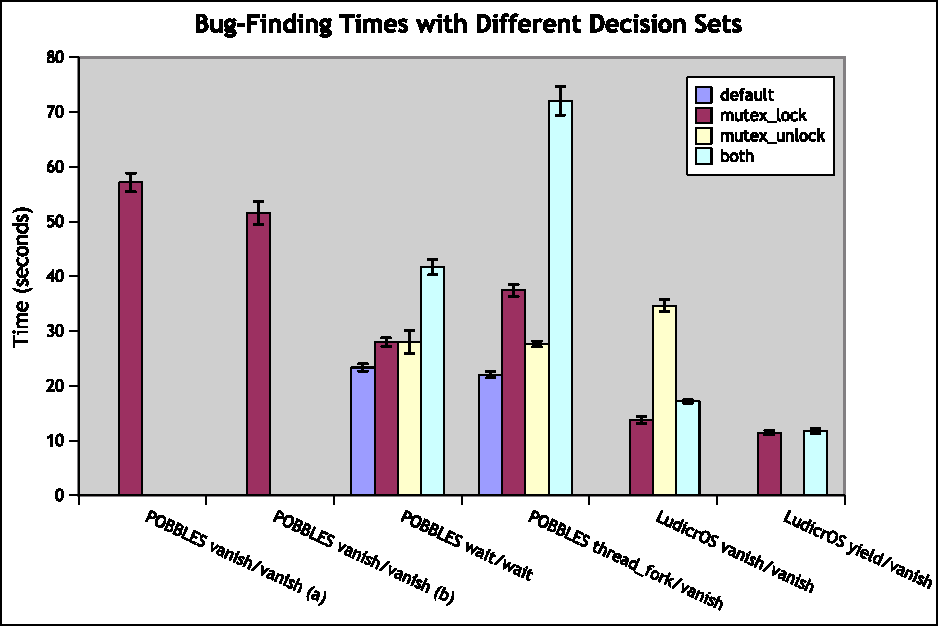
\includegraphics[width=0.7\textwidth]{graphs/decisions.pdf}
	\caption{Bar graph visualisation of the exploration time in trials that did find bugs. The decision trees that did not expose bugs, and the ones that timed out, are not shown.}
	\label{fig:number-graph}
\end{figure}
}

The experimental set-up is as follows:

\begin{itemize}
	\item All Landslide trial times include the Simics start-up and kernel boot-up time (time between issuing the command and the test case beginning to run), roughly 15 seconds for POBBLES and 10 seconds for LudicrOS.
	\item All Landslide trials were run on the Gates-Hillman cluster machines (2.6 GHz Xeon; \revision{four cores, though only one was used; 8 GB RAM}).
	\item All Landslide trials were run with ``backwards exploration'' enabled (Section~\ref{sec:using-search}).
	\item All trials were also run with Landslide configured to pay attention to only the relevant system calls (using \texttt{within\_function}; Section~\ref{sec:using-decision}).

	We believe it is reasonable to test for these bugs in this way (using the minimal set of system calls to be paid attention to as necessary to find the bug) because it follows the recommended workflow of using Landslide, which is to start with what the user judges to be the ``smallest relevant set'' of decision points. The configuration using \texttt{within\_function} was as follows.
	{\small
	\begin{itemize}
		\item POBBLES vanish/vanish(a): \texttt{within\_function vanish}
		\item POBBLES vanish/vanish(b): \texttt{within\_function vanish}
		\item POBBLES wait/wait: \texttt{within\_function wait}
		\item POBBLES thread\_fork/vanish: \texttt{within\_function thread\_fork} and \texttt{within\_function vanish}
		\item LudicrOS vanish/vanish: \texttt{within\_function vanish}
		\item LudicrOS yield/vanish: \texttt{within\_function yield} and \texttt{within\_function vanish}
	\end{itemize}
	}
\end{itemize}

%The stress test experimental set-up is as follows:
%
%\begin{itemize}
%	\item A wrapper program runs 1024 simultaneous copies of the same test program that Landslide uses. Whenever one of them exits, the wrapper starts a new one.
%	\item All stress test trials are on on the ``412 lab crashbox'' (3.2 GHz Pentium D).
%	\item The kernel and test case are configured to not print any messages during the test
%\end{itemize}

%%%%

\newcommand\bugtree[1]{\textcolor{BrickRed}{\bf #1}}
\newcommand\nobugtree[1]{\textcolor{Blue}{[{\em #1}]}}
\begin{table}[t!]
	\begin{center}
	\footnotesize
	\begin{tabular}{|l|l||c|c|c|c|}
		\hline
		\multirow{2}{*}{\bf Kernel and test case} & \multirow{2}{*}{\bf Property of tree} & \multicolumn{4}{|c|}{\bf Decision points used} \\
		\cline{3-6}
		& & \bf default & \bf lock & \bf unlock & \bf both \\
		\hline\hline
		\multirow{4}{*}{POBBLES vanish/vanish (a)} & Decision points & \nobugtree{56} & \bugtree{1296} & N/A & N/A \\
		& Total backtracks   & \nobugtree{16} & \bugtree{376} & N/A & N/A \\
		& Average branch depth & \nobugtree{5} & \bugtree{19} & N/A & N/A \\
		\hline
		\multirow{4}{*}{POBBLES vanish/vanish (b)} & Decision points & \nobugtree{56} & \bugtree{1295} & \nobugtree{382071} & N/A \\
		& Total backtracks   & \nobugtree{16} & \bugtree{376} & \nobugtree{112706} & N/A \\
		& Average branch depth & \nobugtree{5} & \bugtree{17} & \nobugtree{16} & N/A \\
		\hline
		\multirow{4}{*}{POBBLES wait/wait} & Decision points & \bugtree{23} & \bugtree{102} & \bugtree{74} & \bugtree{378} \\
		& Total backtracks   & \bugtree{4} & \bugtree{17} & \bugtree{12} & \bugtree{56} \\
		& Average branch depth & \bugtree{6} & \bugtree{10} & \bugtree{9} & \bugtree{14} \\
		\hline
		\multirow{4}{*}{POBBLES thread\_fork/vanish} & Decision points & \bugtree{24} & \bugtree{394} & \bugtree{273} & \bugtree{2269} \\
		& Total backtracks   & \bugtree{5} & \bugtree{70} & \bugtree{56} & \bugtree{410} \\
		& Average branch depth & \bugtree{5} & \bugtree{16} & \bugtree{14} & \bugtree{23} \\
		\hline
		\multirow{4}{*}{LudicrOS vanish/vanish} & Decision points & \nobugtree{10} & \bugtree{16} & \bugtree{141} & \bugtree{42} \\
		& Total backtracks   & \nobugtree{2} & \bugtree{3} & \bugtree{48} & \bugtree{10} \\
		& Average branch depth & \nobugtree{2} & \bugtree{7} & \bugtree{9} & \bugtree{14} \\
		\hline
		\multirow{4}{*}{LudicrOS yield/vanish} & Decision points & \nobugtree{8} & \bugtree{5} & \nobugtree{149} & \bugtree{7} \\
		& Total backtracks   & \nobugtree{1} & \bugtree{0} & \nobugtree{43} & \bugtree{0} \\
		& Average branch depth & \nobugtree{2} & \bugtree{0} & \nobugtree{9} & \bugtree{0} \\
		\hline
	\end{tabular}
	\end{center}
	\caption{Information about the decision trees explored when finding bugs. As in the previous table, each test case was run with the four different sets of decision points. ``\nobugtree{X}'' means the tree was completely explored because Landslide did not find a bug in that configuration. ``\bugtree{X}'' reflects the portion of the tree that was explored before a bug was found.}
	\label{fig:trees}
\end{table}

Table~\ref{fig:trees} presents more detailed information about the decision trees that Landslide explored when finding these bugs.
For each set of decision points on each bug, we give the total number of decision points in the tree, the total number of backtracks (i.e. branches explored before the bug was found), and the average branch depth (i.e. number of decision points in each branch).

%%%%%%%%%%%%%%%%%%%%%%%%%%%%%%%%%%%%%%%%%%%%%%%%%%%%%%%%%%%%%%%%%%%%%%%%%%%%%%%%
%\section{Summary of Bugs Found}

% FIXME

%%%%%%%%%%%%%%%%%%%%%%%%%%%%%%%%%%%%%%%%%%%%%%%%%%%%%%%%%%%%%%%%%%%%%%%%%%%%%%%%
\section{Discussion}

\subsection{Invariants}

While evaluating Landslide on these bugs, we determined two invariants that must hold for multiple explorations on the same test case.

\begin{enumerate}
	\item {\bf Ordering invariant.} For a given set of decision points, exploring the tree in multiple different orders (``forwards''/``backwards'') should produce the same result in terms of whether a bug was found or not. The bugs found may be different, and the number of branches explored may be different, but it should never be that one ordering finds a bug while another ordering of the same tree finds no bug.
	\item {\bf Superset invariant.} For a given set of decision points, if an exploration of the resulting tree finds a bug, using a superset of that set of decision points should also find a bug. This is because the first tree will be a sub-tree of the second, as shown by never preempting at a decision point that appears in the second set but not the first.
\end{enumerate}

In short, even though Landslide may give false negatives from using imperfect sets of decision points, the exploration itself must be sound (i.e. not missing any bugs that exist in the resulting tree).

When running LudicrOS yield/vanish with decision points on \texttt{mutex\_unlock} but not on \texttt{mutex\_lock}, we found that the ordering invariant failed: ``backwards'' exploration found no bug, while ``forwards'' exploration did. We attribute this to a bug in Landslide itself, and present the results for the backwards exploration as usual, in which Landslide found no bug.

\subsection{Recommended Testing Strategies}
\label{sec:discussion-strategies}

We make several observations about the experimental results from Section~\ref{sec:eval-numbers}.

\begin{enumerate}
	\item {\bf Fewer is faster.} While it is theoretically possible that a tree built of finer-grained interleavings might encounter a bug after fewer overall backtracks, we found that this did not happen in practice.\footnote{
		The one suspicious case is the LudicrOS vanish/vanish bug. Exploring the ``both'' tree found the bug faster than exploring the ``unlock'' tree, despite the latter's decision points being a subset of the former's. However, we see that exploring the ``lock'' tree found the bug faster than either, so overall the ``both'' tree did not outperform the fastest of the smaller trees.}
		In general, for two sets of decision points that both find the same bug, the one that results in shorter {\em branches} will result in fewer {\em backtracks} needed to expose the bug, and hence less overall time.
	\item {\bf Different decision points are differently likely to expose different bugs.} We see that even though the ``lock'' and ``unlock'' trees tended to be about the same size, they were each sometimes better than the other at finding bugs. The ``lock'' tree did better on the vanish/vanish bugs and the yield/vanish bug, while the ``unlock'' tree did better on the wait/wait bug and the thread\_fork/vanish bug.\footnote{
	The latter two bugs needed no more than the default set to uncover at all, but we claim this still demonstrates the principle in general.}
	\item {\bf Finding a bug is fast, if it exists.} As especially exhibited in the POBBLES vanish/vanish (b) case, if two sets of decision points generate trees of approximately equal size, but one tree contains a bug and the other doesn't, then searching the bugful tree will likely terminate much more quickly.
	Of course, it is always possible that a bug may exist only in the very last branch of a tree, but we found that in general bugs show up early during exploration.
\end{enumerate}

% TODO: Investigate the tree size that bugs did exist in. Investigate how many buggy branches there were.

In light of these, we recommend several principles to govern an overall strategy to automatically iterate through different sets of decision points in search of a bug.\footnote{
We now say ``Landslide'' here to refer to a hypothetical test framework to embody these strategies, although of course it would not have to be named that.}

\begin{enumerate}
	\item {\bf Iterate exploring, starting with smaller decision sets.} To properly test for a bug in a particular test case, Landslide should try as many different decision sets as possible.
	The first exploration should always be just the default decision set, because that tends to complete quickly, and can help identify new decision points (Section~\ref{sec:future-analysis}).
	When Landslide has multiple decision sets as candidates for the next exploration, it should prefer to explore ones that result in shorter average branch depth.
	In this way, Landslide will tend to find bugs with the minimal decision set needed to expose them, in accordance with observation 1 above.
	\item {\bf Run multiple explorations at once.}
	As per observation 2, if Landslide has two decision sets that result in roughly equal average branch depth, it cannot know in advance whether either one will find a bug and/or finish significantly faster than the other. As such, it should try to run both explorations in parallel, wait for either one to finish, and continue iterating as appropriate even if the other one has not finished.
	\item {\bf De-prioritise longer-lasting test configurations.}
	With finite resources for parallelisation, Landslide should attempt to load-balance whatever searches are running in parallel according to each one's likelihood of finding a bug.
	In light of observation 3, if a particular search is running abnormally long for its average branch depth (the POBBLES vanish/vanish (b) bug with the ``unlock'' tree is a prime example), Landslide could judge that it is less likely to end soon with a positive result, and prioritise searches with other decision sets.
\end{enumerate}

% vim: ft=tex

%%%%%%%%%%%%%%%%%%%%%%%%%%%%%%%%%%%%%%%%%%%%%%%%%%%%%%%%%%%%%%%%%%%%%%%%%%%%%%%%
\chapter{Future Work}
%%%%%%%%%%%%%%%%%%%%%%%%%%%%%%%%%%%%%%%%%%%%%%%%%%%%%%%%%%%%%%%%%%%%%%%%%%%%%%%%
\label{sec:future}

As Landslide is an experimental foray into the world of systematic exploration in kernel-space, and a detailed study of systematic exploration in general, it has opened up many avenues for potential future improvements.

%%%%%%%%%%%%%%%%%%%%%%%%%%%%%%%%%%%%%%%%%%%%%%%%%%%%%%%%%%%%%%%%%%%%%%%%%%%%%%%%
\section{Interface Improvements}
\label{sec:future-interface}

In Section~\ref{sec:eval-feedback}, we describe many ways in which Landslide's user interface is lacking. These improvements would not necessarily be research developments, but would enhance the user experience in ways necessary for continuing work in the context of 15-410.\footnote{
Landslide is also missing functionality to automatically identify decision points when newly-forked threads become runnable but not immediately switched to. This was not necessary to find the \texttt{double\_thread\_fork} bug in POBBLES (Section~\ref{sec:eval-casestudy}) only because POBBLES automatically switched to the child thread immediately.}

\begin{itemize}
	\item Landslide currently does not support ability to replay a particular choice sequence. If the user finds a bug, and wants to re-execute the interleaving that led to it, they have no choice but to re-explore the tree.
	\item Although Simics can pause execution and give the user a debug prompt, Landslide currently does not support being interrupted during exploration.
		This is because the current implementation uses a wrapper script around the Simics prompt which Landslide communicates with to perform backtracking.
		Though it would be difficult to redesign, it would be good to work around, to enable the user to interrupt, use the Simics debug prompt arbitrarily, and resume Landslide when ready.
	\item Landslide could print its decision traces in a better format. The current format is basically a ``raw data dump''. Raw text is probably the wrong interface; a graphical/tabular format with distinct columns for the execution of each different thread would be easier to understand.
	\item Landslide could attempt to detect when something has gone wrong that is not its fault (such as incorrect instrumentation, or the kernel violating some of its requirements), and print a useful error message rather than behaving mysteriously.
\end{itemize}

%%%%%%%%%%%%%%%%%%%%%%%%%%%%%%%%%%%%%%%%%%%%%%%%%%%%%%%%%%%%%%%%%%%%%%%%%%%%%%%%
\section{Education}
\label{sec:future-education}

\subsection{Landslide as a Teaching Tool}

\begin{figure*}[h]
	\begin{center}
	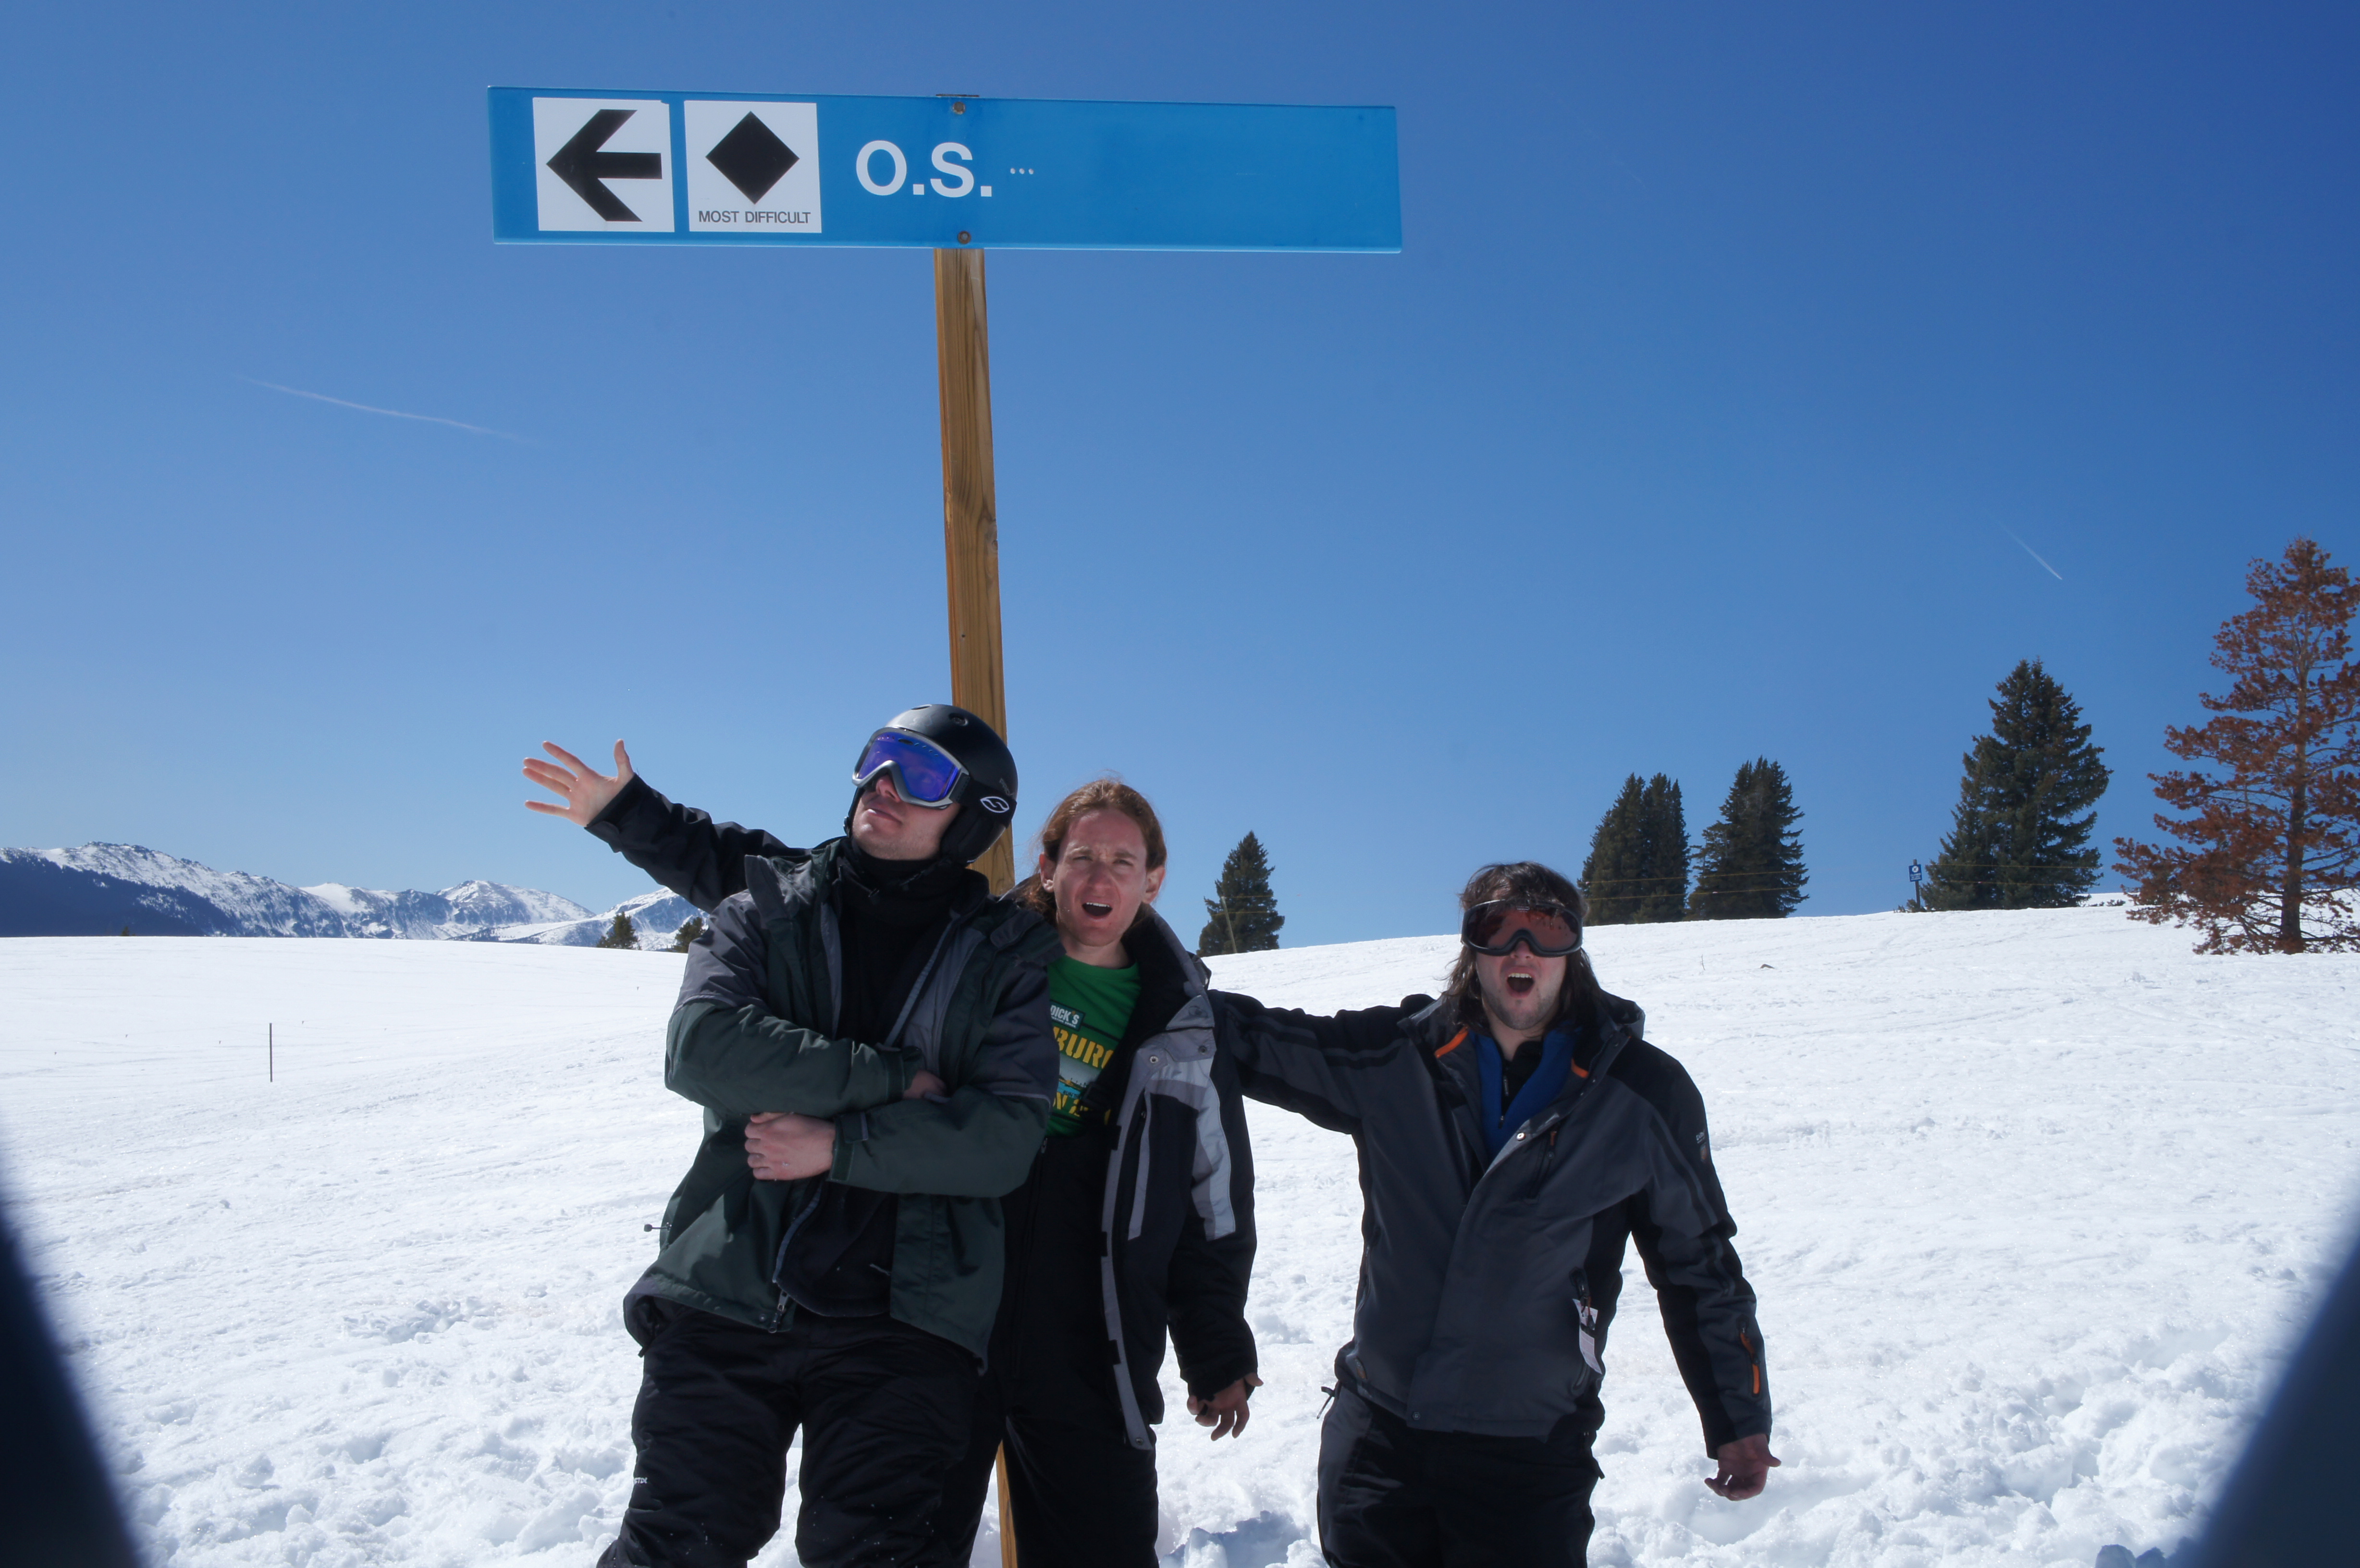
\includegraphics[width=0.75\textwidth]{wont-modify-vail.jpg}
	\end{center}
	\caption{Former members of Operating Systems course staff lament the difficulty involved in teaching students concurrency debugging skills.}
\end{figure*}

15-410 currently teaches students concurrency debugging skills ``the hard way'': by immersing them in environments where races will arise, and letting them find debugging tactics on their own to use in conjunction with conventional stress testing.

We believe that a tool such as Landslide could change the way students learn such skills for the better, beyond simply increasing their likelihood of finding bugs during testing. The decision tree is a much more structured way of expressing a test case's concurrent behaviour than the way 15-410 currently teaches, which is ``think hard until you figure out the buggy interleaving.'' Having students use Landslide, even to a small extent, might encourage them to think in this more structured way.\footnote{
\revision{In 15-410, before the kernel project, students also implement a user-space thread library. Just as Landslide could help the students during the kernel project, so too could a user-space systematic exploration tool help during the thread library project.}}

\subsection{Landslide as a Grading Tool}

The 15-410 grading infrastructure currently uses a program called Fritz, which is a stress testing wrapper around a suite of test programs. Some of these tests are Landslide-friendly (Section~\ref{sec:using-landslide-friendly-tests}), and some are themselves stress tests. The 15-410 course staff also hand-grade every kernel, in part because Fritz is known for only catching race conditions at random and infrequently.

While far from being able to replace talented humans for grading, we believe that, after some improvement, Landslide could augment or replace Fritz as a tool for automatically finding several common patterns of concurrency errors that students have (especially races involving exiting threads, which we have shown Landslide is effective at finding).

\revision{
\subsection{Making Pebbles Landslide-Friendly}

If Landslide becomes integrated into an undergraduate course curriculum, it will be important to minimise the amount of effort students have to go through to instrument their kernels. This could be achieved in part by changing the project definition in ways that make Landslide better able to automatically instrument kernels. For Pebbles, we recommend the following changes.

\begin{enumerate}
	\item {\bf Timer ticks control ``runnable'' threads.} As discussed in Section~\ref{sec:model-timer}. Additionally, to prevent the users from having to instrument non-descheduling mutexes, the project could mandate that all concurrency primitives actually remove blocked threads from the runqueue.
	\item {\bf No idling when progress can be made.} Also as discussed in Section~\ref{sec:model-timer}. With the current specification, inappropriate idling is merely a performance bug, though it is incompatible with Landslide. If the project gave stricter requirements regarding this, fewer students would need to fix problems with their scheduler idling during the instrumentation process.
	\item {\bf Mandated function names for scheduling events.} As part of the instrumentation process, students tell Landslide where in their schedulers notable events happen. Landslide could automatically detect some of these if the project mandated the names of certain functions, such as the timer handler, context switcher, and runqueu manipulation routines.
\end{enumerate}

\subsection{Virtual Memory Bug-Finding}

In this work, we focused especially on races related to the thread lifecycle routines. We believe Landslide would be immediately applicable to certain varieties of virtual memory bugs, but other types might not be easily exposed with Landslide's current model.

For example, one of the groups in the user study said they were looking for a race that only arose in out of memory conditions. A test case that could expose that race, by exhausting the kernel's memory resources, would necessarily have a very large state space that would be impractical to explore systematically.

We suggested to the group to configure their kernel to fail memory allocations every so often, so Landslide would be better able to find the race while still using a small test case. To make Landslide more applicable to such bugs in general, we might further investigate this debugging strategy in a more structured way.
}

%%%%%%%%%%%%%%%%%%%%%%%%%%%%%%%%%%%%%%%%%%%%%%%%%%%%%%%%%%%%%%%%%%%%%%%%%%%%%%%%
\section{New Techniques}
\label{sec:future-new}

Related research in dynamic verification has introduced testing techniques orthogonal to systematic exploration, which could augment its effectiveness if combined in one tool. We discuss the potential for using other techniques in Landslide or in any other systematic testing framework.

\subsection{Data Race Detection}
\label{sec:future-analysis}

Landslide currently never alters its set of decision points once it begins executing. The user must configure the set of decision points in advance, and Landslide follows them to the letter when exploring the tree. This is useful for investigating the size of trees generated by certain sets of decision points, but future work should do better than leaving it up to the user to stumble across a set of decision points that exposes a bug.

Most notably among the information Landslide has at its disposal is the collection of conflicting shared memory accesses among transitions. Theoretically, to identify a decision point immediately before and after each such access would generate an execution tree with perfect granularity (i.e., exactly one shared memory access per transition), and thence find every possible race condition, which would be the opposite extreme to the current setup.

Landslide could make use of data race detection techniques~\cite{datacollider}, however, to strike a middle ground in which shared memory accesses it chooses.
\begin{enumerate}
	\item It should be aware of the types and interfaces associated with the kernel's synchronisation primitives (mutexes, condvars, semaphores, etc), and be able to treat operations on those as ``guaranteed to work'' (similar to Section~\ref{sec:por-independence}).\footnote{
	\revision{If such operations were instead themselves incorrect, it would mean that data race detection might fail to identify certain racy accesses. The technique would then still identify some racy accesses, but might miss others.}}
	\item Next, it should recognise acquire and release (or sleep and wake) operations on synchronisation primitives, and use that information to track lockset-type information.
	\item Ultimately, it should use the lockset information in conjunction with the happens-before relation to identify which memory accesses are ``raciest'', and add decision points around those.
\end{enumerate}

\subsection{Parallelism}

Landslide's tree exploration is implemented sequentially. However, because DPOR's approach of tagging which sibling branches should be explored next generally follows a workqueue-based depth-first-search structure, it should not be too difficult to parallelise. Prior work exists for this technique~\cite{distributed-dpor}, so it would not be a research contribution, but would substantially improve Landslide's effectiveness regardless.

\subsection{Symbolic Execution}
\label{sec:future-dawson}

In Section~\ref{sec:related-orthogonal}, we mentioned the technique of symbolic execution for dynamic verification. We believe that symbolic execution could be combined with systematic exploration to help find races in certain obscure code paths that systematic exploration by itself might not even execute.

One interesting phenomenon that would occur from combining symbolic execution and systematic exploration would be a new notion of decision points. Symbolic execution involves its own state space exploration, in which control flow branch points correspond to decision points; hence, to combine it with systematic exploration would create a hybrid state space in which a ``decision point'' could be a place where either different threads could preempt each other or multiple control flow paths could be taken~\cite{dawson}.

\subsection{Trace Minimisation}
\label{sec:future-trace-minimisation}

Also in Section~\ref{sec:related-orthogonal}, we mentioned related research that attempts to {\em minimise} the set of conditions that are known to be associated with a bug~\cite{dag-mining}.
In the context of Landslide, this corresponds to how easy the decision trace is to understand. Even if Landslide finds a bug and prints the list of thread switches that were made, it may still be very difficult for the user to understand if the list includes many unnecessary switches that were completely unrelated to the bug.

Landslide could continue to be of use even after it has found a bug, by attempting to find a ``minimal decision trace''. It could search different subsets of the known-buggy trace in an attempt to find shorter traces which result in the same bug.
In this way, it would be able to print decision traces that automatically give the programmer much more insight into the true nature of each race condition.

While studying various bugs found by Landslide, we found that in general, when there were frivolous thread switches in the decision trace, users most benefitted from starting to read the trace at the end; i.e., considering the most recent transition made by each thread. Hence, when building a search algorithm for trace minimisation, it would be good to more heavily prioritise decisions that occurred later in a buggy branch.

%%%%%%%%%%%%%%%%%%%%%%%%%%%%%%%%%%%%%%%%%%%%%%%%%%%%%%%%%%%%%%%%%%%%%%%%%%%%%%%%
\section{Linux}
\label{sec:future-linux}

The Linux kernel is a logical next kernel architecture to target with Landslide.

One advantage of targetting Linux is that a testing framework will be able to make assumptions about the scheduler design, in ways that Landslide was not able to (Section~\ref{sec:challenges-design}), because the kernel instrumentation will not need to be repeatedly re-implemented (as it did for each 15-410 student kernel that we tested).

However, Linux is a much more complicated kernel architecture than Pebbles, and we would face several challenges.

\subsection{Multi-Processor Support}

Landslide's way of modelling concurrency as a tree of thread interleavings directly expresses the way concurrency arises on uniprocessor systems. On multiprocessor systems such as Linux, however, there is ``true concurrency'': different threads may be running at the same time on different processors, rather than just interleaved. Hence, race conditions that were previously impossible in a uniprocessor environment may be commonplace in SMP.

In order to support multiprocessor kernels, Landslide would need to refine its representation of the decision tree to express the potential for threads interleaving either on the same processor or on different processors. As a starting point, we note that on SMP, at each decision point, in addition to choosing any of $N$ threads to run, we must choose from among $M$ processors for it to run on.

\subsection{Performance}

Linux is much bigger than a Pebbles kernel (in terms of amount of code that runs during startup, during scheduling, etc), and hence would be much more expensive to test in a simulated environment. We suspect that in order to practically test Linux, we would need to implement systematic exploration in a virtualised environment, which we discuss more in Section~\ref{sec:future-virt}.

\subsection{Complicated Synchronisation Patterns}

Many components of Linux contain ad-hoc synchronisation, often done for performance reasons, which would be difficult to reason about. One common pattern is attempting some operation, checking later if it got interfered with, and rewinding and trying again if so. A straightforward approach to building a decision tree representing this might result in an infinitely deep branch: if the thread that gets interfered with keeps getting selected for scheduling, it would never make any progress. The testing tool would need to recognise these cases, and understand the invisible dependency on ``somebody else'' running first.

\subsection{Device Drivers}
\label{sec:future-drivers}

There is much more device driver code in Linux than there is for its core components, and the device driver code also does not undergo as rigorous code review. Because of this, device drivers are much more prone to concurrency errors than the core components, and hence a systematic exploration framework for Linux should focus on testing them.

However, the concurrency model of device drivers is much more complicated than the simple timer-based scheduling model we used in this work. In addition to timer-driven preemptions, code may also be interleaved as caused by device interrupts and input. Like support for SMP, being able to systematically test for device driver races will also require a more sophisticated representation of the decision tree.

In addition to controlling timer interrupts, a systematic testing tool would also need to control device interrupts and device input, both of which are also nondeterministic inputs to the kernel.
Furthermore, it would need to recognise common components of device drivers to properly cause relevant scheduling patterns, such as the ``top half'' and ``bottom half'' of interrupt handlers and dedicated device driver threads.

These components would all be candidates for being scheduled at a decision point, although it more complicated still than simply choosing from among several threads to run. For example, the bottom half of an interrupt handler would depend on a top half having already executed, and interrupt handlers would run on the same stack as other thread rather than on their own stack.

\revision{Because many driver bugs result from interactions with error-handling paths, it will also help to understand the difference between normal device input and faulty input in order to maximise code path coverage. Symbolic execution (Section~\ref{sec:future-dawson}) may help address this.}

%%%%%%%%%%%%%%%%%%%%%%%%%%%%%%%%%%%%%%%%%%%%%%%%%%%%%%%%%%%%%%%%%%%%%%%%%%%%%%%%
\section{Virtualisation}
\label{sec:future-virt}

Compared to executing the code being tested on real hardware (which tools such as \cite{dbug-ssv} are able to do for user-space programs), Simics is {\em slow}, and even slower with Landslide hooked up to it.

Major benefit could be achieved by redesigning Landslide to work in a virtualised environment instead of a simulated one. This would pose several challenges, because Landslide would no longer be running in ``\revision{omniscient} mode'', having immediate access to every single instruction and memory access executed. It would, however, still be able to modify the kernel's memory and address space, which would be important to harness for increased control over the kernel's execution.

We speculate on some challenges and potential solutions that virtualised execution might have to offer. We assume that our users will be talented kernel developers rather than undergraduate students, and hence allow for more complicated interface requirements.

\subsection{Interposition}

\subsubsection{Event Tracking}

The event-based nature of the \texttt{tell\_landslide} annotations can still be harnessed in a virtualised environment. They would need to be converted into hypercalls, which would briefly transfer control to Landslide at key execution points to enable it to update its state machine and potentially influence the kernel's execution.

We would add additional \texttt{tells\_landslide} for the kernel components which are presently automatically instrumented, such as the dynamic memory allocator and the \texttt{panic} routines, and also for certain components that are currently instrumented with \texttt{config.landslide}, such as identifying when the context switcher returns or when the timer interrupt handler is invoked.

Rather than using the schedule-in-flight algorithm, Landslide could simplify its job by asking the kernel to run a particular thread directly, as described in Section~\ref{sec:components-inflight}.

\subsubsection{Memory Tracking}

More challenging than tracking important kernel events will be tracking all accesses to shared memory. We could exploit the virtualised virtual memory system, and write-protect (possibly also read-protect, i.e., unmap) all pages that contain shared data, such as the global data section and the dynamic allocation heap. All accesses would then page-fault, transferring control to Landslide.

\subsection{Backtracking}

Simics's convenient bookmarking mechanism will be no more in virtual-machine-land. One possibility for backtracking would be to record-and-replay the events of each branch (up to the point at which Landslide chooses to have decided differently), restarting the system's execution from the beginning each time. Another option might be to snapshot the state of the kernel at each decision point, and use those to resume without re-executing everything from the beginning (kernel boot-up and initialisation is much more expensive than individual system calls, after all).

\subsection{Control over Non-Determinism}

Finally, Landslide will need to find new ways to control non-deterministic events in the system. Since virtualised kernels use the same timer interrupt as the host they run on, Landslide \revision{will need to intercept it, and perhaps control the guest kernel's context switching with a custom ``Landslide-driven'' context switcher instead.}

Likewise, Landslide will need to control other non-deterministic inputs to the kernel, including device interrupts/input and even the system clock.

%%%%%%%%%%%%%%%%%%%%%%%%%%%%%%%%%%%%%%%%%%%%%%%%%%%%%%%%%%%%%%%%%%%%%%%%%%%%%%%%
\section{Long-Running Test Shaping}
\label{sec:future-shaping}

Another area to investigate is that of systems which could be tested continuously. Instead of the goal of finishing exploring a test case without finding a bug, a long-running testing approach would focus on ``shaping'' the test configuration to more and more refined configurations in hopes of finding a bug eventually.

In Section~\ref{sec:discussion-strategies}, we recommend an iteration strategy to effectively explore trees with multiple different sets of decision points, while not knowing ahead of time which, if any, may contain a bug.
This strategy would give rise to a test framework which could explore multiple different types and granularities of interleavings at once, heuristically judge which are more likely to uncover bugs, and prioritise resource allocation and search direction accordingly.

There is also the question of when during the testing process new decision points should be introduced.
One possibility would be to begin exploration with a small set of decision points, explore the resulting tree, analyse the tree post-hoc to identify additional decision points, and iterate exploring with the new set.
Another possibility would be to identify decision points along the way, analysing each branch of the tree after executing it, to generate the decision points for that very branch, and thence use them to find which branch to explore next.
It remains to be seen which approach would be more effective.

\revision{One possible application of such a strategy would be in searching for bugs given only a stack trace and/or kernel log from a crash report. The components of the kernel mentioned in the trace or log could be used as the initial focus for the test, and the framework could gradually expand its scope to search for an interleaving granularity which would reproduce the bug.}

%%%%%%%%%%%%%%%%%%%%%%%%%%%%%%%%%%%%%%%%%%%%%%%%%%%%%%%%%%%%%%%%%%%%%%%%%%%%%%%%
\section{Theoretical Oddities}
\label{sec:future-theory}

During our in-depth case studies, we noticed two interesting properties about certain decision trees. We believe these warrant further theoretical study, to better understand the nature of these decision trees. This may in turn give rise to heuristics for making systematic testing more effective.

% TODO: make visualisations for both of these
\subsection{``Backwards'' Exploration}
\label{sec:future-backwards}

\revision{
\renewcommand\bugnum[2]{#1 {\scriptsize \em (#2)}}
\begin{table}[t]
	\centering
	\footnotesize
	\begin{tabular}{|l|l||c|c|c|}
	\hline
	{\bf Bug} & {\bf Direction} & {\bf Time} & {\bf Backtracks} & {\bf Trace Length} \\
	\hline\hline
	\multirow{2}{*}{POBBLES vanish/vanish (a)} & Forwards & \bugnum{124.8}{4.9} & 1264 & 7 \\
	& Backwards & \bugnum{57.1}{1.7} & 376 & 11 \\
	\hline
	\multirow{2}{*}{POBBLES vanish/vanish (b)} & Forwards & \bugnum{106.3}{5.7} & 1030 & 7 \\
	& Backwards & \bugnum{51.5}{2.1} & 376 & 10 \\
	\hline
	\multirow{2}{*}{POBBLES wait/wait} & Forwards & \bugnum{62.6}{3.4} & 132 & 8 \\
	& Backwards & \bugnum{27.9}{0.8} & 17 & 13 \\
	\hline
	\multirow{2}{*}{POBBLES thread\_fork/vanish} & Forwards & \bugnum{21.4}{0.7} & 0 & 6 \\
	& Backwards & \bugnum{37.4}{1.1} & 70 & 6 \\
	\hline
	\multirow{2}{*}{LudicrOS vanish/vanish} & Forwards & \bugnum{14.7}{0.9} & 4 & 3 \\
	& Backwards & \bugnum{13.7}{0.7} & 3 & 7 \\
	\hline
	\multirow{2}{*}{LudicrOS yield/vanish} & Forwards & \bugnum{13}{0.9} & 3 & 3 \\
	& Backwards & \bugnum{11.4}{0.4} & 0 & 5 \\
	\hline
	\end{tabular}
	\caption{Comparison of forwards and backwards explorations for the six case study bugs (using decision points on \texttt{mutex\_lock} but not \texttt{mutex\_unlock}).}
	\label{fig:backwards}
\end{table}
\begin{figure}[h]
	\centering
	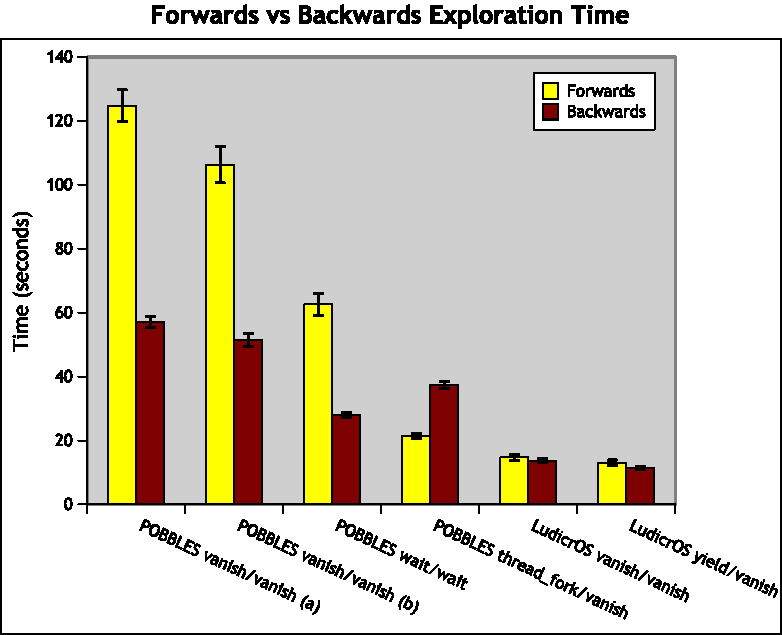
\includegraphics[width=0.47\textwidth]{graphs/backwards-time.pdf}
	\hspace{0.02\textwidth}
	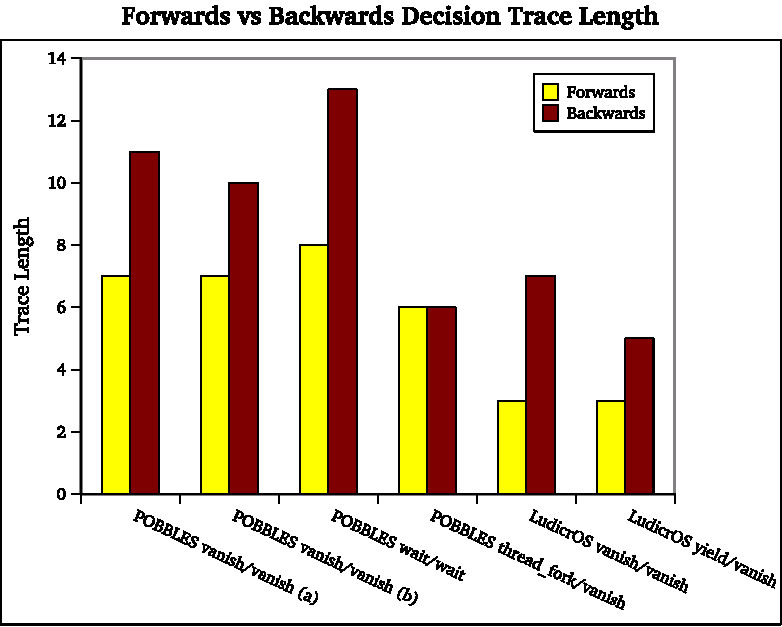
\includegraphics[width=0.48\textwidth]{graphs/backwards-trace.pdf}
	\caption{In general, backwards exploration finds bugs faster, but forwards exploration produces shorter (more understandable) decision traces.}
	\label{fig:backwards-graphs}
\end{figure}
}

We configured Landslide to be able to explore trees in two different orderings, and we found that the two orderings behaved substantially differently in terms of time taken to find bugs and length of decision traces produced.

\begin{itemize}
	\item {\bf Forwards exploration.} When exploring the tree ``forwards'', at each decision point the explorer would choose the currently-running thread if it hadn't already been explored. This resulted in preference for branches of the tree with fewer forced preemptions; the first branch to be explored would have no preemptions at all, and subsequent branches would have generally (but not monotonically) increasing numbers of preemptions.

		Compared to backwards exploration, we found that forwards exploration tended to produce much shorter decision traces for the same bugs. These shorter traces would have fewer thread switches that were irrelevant to the bug itself, and hence be much easier to understand.
	\item {\bf Backwards exploration.} When exploring ``backwards'', at each decision point the explorer would prefer to choose a thread that required a forced preemption. This resulted in preference for branches with more forced preemptions, and the first branch to be explored would have a preemption at every decision point.\footnote{
		This property of backwards exploration is what resulted in the LudicrOS yield/vanish bug being found without any backtracks.}

		Compared to forwards exploration, we found that backwards exploration tended to find bugs much more quickly, with fewer backtracks needed before the buggy branch was chosen.
\end{itemize}

\revision{Table~\ref{fig:backwards} and Figure~\ref{fig:backwards-graphs} compare the tree explorations and resulting decision traces. The one exception is the POBBLES thread\_fork/vanish bug, which Landslide found immediately during forwards exploration, because the race actually required no forced preemptions to expose.}

Compared to Iterative Context Bounding~\cite{chess}, which is based on the insight that bugs need fewer forced preemptions to expose, we believe that our insight is orthogonal. The ICB insight results in smaller decision trees overall needing to be explored before bugs appear, while our insight determines exploration ordering once the tree is constructed.

We are not sure if combining these two insights is possible. In future work we might compare them and investigate this possibility, to determine a heuristic for what exploration orderings are most likely to expose bugs with the fewest needed preemptions.

\subsection{Exploration Tree Structure}
\label{sec:future-nadim}

One member of Group 1 from the user study fully explored decision trees from \texttt{double\_wait} and \texttt{vanish\_vanish} (Section~\ref{sec:eval-victory}), and found an oddity in the exploration time for a particular decision set.

When using decision points on just \texttt{mutex\_lock} or \texttt{mutex\_unlock}, the explorations for each test case took similar time. However, when using decision points on both mutex functions, \texttt{double\_wait} took substantially longer, despite the tree structure suggesting they should have been comparable, with \texttt{double\_wait} even being perhaps slightly faster. Figure~\ref{fig:nadim-stats} shows a comparison of the tree anatomy for these two test cases.

\begin{table}[h]
	\small
	\centering
	\begin{tabular}{|l||c|c|}
		\hline
		& \texttt{double\_wait} & \texttt{vanish\_vanish} \\
		\hline\hline
		Exploration time & {\bf 30 minutes} & {\bf 5 minutes} \\
		\hline
		Backtracks & {\bf 1,401} & {\bf 1,511} \\
		\hline
		Decision points & 10,355 & 5,690 \\
		\hline
		Average branch depth & 18.34 & 16.00 \\
		\hline
		Average instructions/branch& 1,975,033 & 1,984,249 \\
		\hline
		Total instructions & 206,757,601 & 24,907,516 \\
		\hline
		Backtrack distance minimum & {\bf 6} & {\bf 2} \\
		\hline
		Backtrack distance maximum & 17 & 16 \\
		\hline
		Backtrack distance average & {\bf 7.38}  & {\bf 3.75} \\
		\hline
		% FIXME: add stddev?
	\end{tabular}
	\caption{Comparison of expensive \texttt{double\_wait} test and cheap \texttt{vanish\_vanish} test. The number of branches and depth of each branch are similar, but \texttt{double\_wait}'s backtracks were significantly longer, causing more total instructions to be executed.}
	\label{fig:nadim-stats}
\end{table}

Despite the two trees having nearly equal numbers of branches and instructions executed per branch, \texttt{double\_wait} took significantly more time. This is because Landslide's backtracks during \texttt{double\_wait} were significantly {\em longer} than the backtracks in \texttt{vanish\_vanish} on average; i.e., the backtracks were targetting an earlier point during the test's execution.
Hence, Landslide had to execute more total instructions overall to explore the longer branches in \texttt{double\_wait}.\footnote{
Of note, if backtracking had been implemented by restarting the test each time; i.e., executing the full depth of every branch from the root of the tree, the repeated work would have caused the execution times to be equal. The fact that Simics's backtracking avoids the cost of execution that happened before the backtrack target is to credit for this discrepancy.}
% as visualised in figure\ldots TODO

This suggests that the ``interesting'' parts of \texttt{double\_wait} were earlier in the test case, whereas in \texttt{vanish\_vanish} they are more towards the end. We conjecture that, with theoretical study of these structural properties, we could develop search heuristics for focusing on the ``interesting'' parts of the trees, and avoid repeating the irrelevant instructions at the end of each branch.

%%%%%%%%%%%%%%%%%%%%%%%%%%%%%%%%%%%%%%%%%%%%%%%%%%%%%%%%%%%%%%%%%%%%%%%%%%%%%%%%
\chapter*{Acknowledgements}
%%%%%%%%%%%%%%%%%%%%%%%%%%%%%%%%%%%%%%%%%%%%%%%%%%%%%%%%%%%%%%%%%%%%%%%%%%%%%%%%
% Save this for last :)

Thanks to Deb Cavlovich, for holding on to this thesis for a few days more for Ben to finish it properly.

Thanks to my advisor, too, I guess, and maybe also to the people I worked with and my friends as well.

Thanks to the members and companies of the PDL Consortium (including Actifo,
APC, EMC, Emulex, Facebook, Fusion-io, Google, Hewlett-Packard, Hitachi, Huawei
Technologies, Intel, Microsoft, NEC, NetApp, Oracle, Panasas, Riverbed,
Samsung, Seagate, STEC, Symantec, VMware, and Western Digital) for their
interest, insights, feedback, and support.


\bibliography{citations}{}
\bibliographystyle{alpha}

\end{document}
